% ChronicleHeritage -- Major Project Part 1 report (single self-contained file).
% Compile with pdfLaTeX; needs only cbit.png and the images/ folder next to this file.
%
% EDIT THE AUTHOR NAMES AND ROLL NUMBERS IN THE "Editables" BLOCK BELOW BEFORE SUBMITTING.
\documentclass[a4paper,12pt,oneside]{book}
\usepackage[utf8]{inputenc}
\usepackage{amssymb}
\usepackage{amsmath}
\usepackage{graphicx}
\graphicspath{ {images/} }
\usepackage{times}
\usepackage{geometry}
\usepackage{setspace}
\usepackage{tocloft}
\usepackage{fancyhdr}
\usepackage{float}
\usepackage{booktabs}
\usepackage{array}
\usepackage{multirow}
\usepackage{longtable}
\geometry{a4paper, tmargin=1in, rmargin=1in, bmargin=1in, lmargin=1.5in}


%-----------------------------------------
% Editables of the document
%-----------------------------------------
\newcommand{\thesistitle}{ChronicleHeritage: An AI-Driven Digital Twin and Threat-Assessment Platform for Monitoring Indian Heritage Monuments} % Title of the Thesis, change here
\newcommand{\thesisauthora}{Ch. Jyothi (1601-23-771-004)} % Person 1
\newcommand{\thesisauthorb}{N. Sharanya (1601-23-771-014)} % Person 2
\newcommand{\thesisauthorc}{Y. Charan Sai (1601-23-771-303)} % Person 3
% If the number of people is different, change accordingly in titlepage and bonafide-certificate
\newcommand{\thesisdept}{Artificial Intelligence and Data Science} % Department
\newcommand{\thesisguide}{Ms. P. Kiranmaie}
\newcommand{\thesisguidedesig}{Assistant Professor} % Project Guide
\newcommand{\depthod}{Prof. K. Radhika} % Department Head
% Also, change the graduation year in titlepage and bonafide certificate
%-----------------------------------------


% For Figures and Subfigures
\usepackage{graphicx, caption, subcaption}

% Package to keep images in place
\usepackage{float}

% Package for Appendices
\usepackage{titletoc}
\usepackage{appendix}

% Chapter and Appendix in TOC prefixed
\makeatletter
\titlecontents{chapter}%
 [0pt]%
 {\bfseries}%
 {\MakeUppercase \@chapapp\ \thecontentslabel\quad}%
 {}%
 {\normalfont\cftdotfill{\cftdotsep}\contentspage}%
 [\addvspace{0pt}]%

\g@addto@macro\appendices{%
  \addtocontents{toc}{\protect\renewcommand{\protect\@chapapp}{\appendixname}}%
}
\makeatother


% Package for codes
\usepackage{listings}
\lstset{
    breaklines = true,
    captionpos = b,
    numberstyle = \scriptsize,
    numbers=left,
    numbersep=10pt
}


% Package for enumerate
\usepackage{enumitem}

% Block Diagram Packages and Functions
\usepackage{tikz}
\usetikzlibrary{arrows, decorations.markings}
\usetikzlibrary{arrows,positioning,shapes.geometric}
\usetikzlibrary{arrows.meta}
\tikzstyle{vecArrow} = [thick, decoration={markings,mark=at position
   1 with {\arrow[semithick]{open triangle 60}}},
   double distance=1.4pt, shorten >= 5.5pt,
   preaction = {decorate},
   postaction = {draw,line width=1.4pt, white,shorten >= 4.5pt}]
\tikzstyle{innerWhite} = [semithick, white,line width=1.4pt, shorten >= 4.5pt]
\tikzstyle{block} = [draw, fill=blue!20, rectangle,
    minimum height=3em, minimum width=6em]

% Chapter Title Customization
\usepackage{titlesec}
\titleformat{\chapter}[display]
{\Large\bfseries\centering}{\MakeUppercase\chaptertitlename\ \thechapter}{5pt}{\Large}
\titlespacing*{\chapter}{0pt}{0pt}{20pt}

% Section Customization
\titleformat{\section}{\large \bfseries}{\thesection}{1em}{}

% Sub-Section Customization
\titleformat{\subsection}{\fontsize{13pt}{13pt} \bfseries}{\thesubsection}{1em}{}


% Align the titles of auxiliary content to center
\renewcommand*\contentsname{\Large \centerline{TABLE OF CONTENTS}}
\renewcommand*\listfigurename{\Large \centerline{LIST OF FIGURES}}
\renewcommand*\listtablename{\Large \centerline{LIST OF TABLES}}

% tocloft puts 50pt above the TOC/LOT/LOF titles by default; start them at the top of the
% page like every other \chapter* heading (titlesec: 0pt before, 20pt after, \Large bold)
\renewcommand{\cfttoctitlefont}{\Large\bfseries}
\renewcommand{\cftlottitlefont}{\Large\bfseries}
\renewcommand{\cftloftitlefont}{\Large\bfseries}
\setlength{\cftbeforetoctitleskip}{0pt}
\setlength{\cftbeforelottitleskip}{0pt}
\setlength{\cftbeforeloftitleskip}{0pt}
\setlength{\cftaftertoctitleskip}{20pt}
\setlength{\cftafterlottitleskip}{20pt}
\setlength{\cftafterloftitleskip}{20pt}

% Table captions go above the table (figure captions stay below)
\captionsetup[table]{position=top}


% Page Style
\pagestyle{fancy}
\cfoot{\thepage}
\rhead{}
\lhead{}
\renewcommand{\headrulewidth}{0pt}
\renewcommand{\footrulewidth}{0pt}

% Line Spacing
\usepackage{setspace}

% Indent First Paragraph
\usepackage{indentfirst}

% To make uppercase words
\usepackage{textcase}


\usepackage{url}
\usepackage[bookmarks, colorlinks=false, pdfborder={0 0 0}, pdftitle={\thesistitle}, pdfkeywords={}]{hyperref}


\begin{document}

% To expand the word spacing
\spaceskip=1.5\fontdimen2\font plus 1.5\fontdimen3\font
minus 1.5\fontdimen4\font


\frontmatter
\pagenumbering{gobble}
% ===== titlepage =====
\begin{titlepage}
\begin{center}
\fontsize{18pt}{1cm}\selectfont \textbf{\thesistitle}

\vspace*{0.8cm}
\fontsize{14pt}{21pt}\selectfont A Report on Major Project Part 1 \\
submitted in partial fulfillment of the requirements for \\
the award of the degree of

\vspace*{0.3cm}
\fontsize{14pt}{1cm}\selectfont\textbf{Bachelor of Engineering}

\vspace*{0.3cm}
\textbf{in\\\thesisdept}

\vspace*{0.5cm}
By

\textbf{\thesisauthora}\\
\textbf{\thesisauthorb}\\
\textbf{\thesisauthorc}\\
\vspace*{0.5cm}
\textbf{\textit{Under the esteemed guidance of}}\\
\textbf{\thesisguide}\\
\thesisguidedesig\\
\vfill

\includegraphics[width=1.25in]{cbit.png}

\vspace*{0.3in}
\fontsize{12pt}{12pt}\selectfont \textbf{DEPARTMENT OF ARTIFICIAL INTELLIGENCE AND DATA SCIENCE}\\[0.2cm]
\fontsize{14pt}{14pt}\selectfont\textbf{CHAITANYA BHARATHI INSTITUTE OF TECHNOLOGY}\\[0.2cm]
\textbf{HYDERABAD -- 500075}

\vspace*{0.2cm}
\textbf{NOVEMBER 2026}
\end{center}
\end{titlepage}

% ===== vision / mission =====
\thispagestyle{empty}
\begin{center}

\includegraphics[width=1.0in]{cbit.png}

\vspace*{0.3in}
\fontsize{12pt}{12pt}\selectfont \textbf{DEPARTMENT OF ARTIFICIAL INTELLIGENCE AND DATA SCIENCE}\\[0.2cm]
\fontsize{14pt}{14pt}\selectfont\textbf{CHAITANYA BHARATHI INSTITUTE OF TECHNOLOGY}\\[0.2cm]
\textbf{HYDERABAD -- 500075}\\
\vspace*{0.3in}
\fontsize{16pt}{16pt}\textbf{INSTITUTE VISION}
\end{center}

\vspace{0.05cm}
\noindent
\fontsize{10pt}{24pt}\selectfont ``To be the center of excellence in technical education and research''.

\begin{center}
\fontsize{16pt}{16pt}\textbf{INSTITUTE MISSION}
\end{center}

\vspace{0.05cm}
\noindent
\fontsize{10pt}{24pt}\selectfont ``To address the emerging needs through quality technical education and advanced research''.

\vspace{0.05cm}

\begin{center}
\fontsize{16pt}{16pt}\textbf{DEPARTMENT VISION}
\end{center}

\vspace{0.05cm}
\noindent
\fontsize{10pt}{24pt}\selectfont ``To be a globally recognized center of excellence in the field of Artificial Intelligence and Data Science that produces innovative pioneers and research experts capable of addressing complex real-world challenges and contributing to the socio-economic development of the nation.''

\begin{center}
\fontsize{16pt}{16pt}\textbf{DEPARTMENT MISSION}
\end{center}

\vspace{0.05cm}
\noindent
\fontsize{10pt}{24pt}\selectfont
\begin{enumerate}
    \item To provide cutting-edge education in the field of Artificial Intelligence and Data Science that is rooted in ethical and moral values.
    \item To establish strong partnerships with industries and research organizations in the field of Artificial Intelligence and Data Science, and to excel in the emerging areas of research by creating innovative solutions.
    \item To cultivate a strong sense of social responsibility among students, fostering their inclination to utilize their knowledge and skills for the betterment of society.
    \item To motivate and mentor students to become trailblazers in Artificial Intelligence and Data Science, and develop an entrepreneurial mindset that nurtures innovation and creativity.
\end{enumerate}

\newpage

\clearpage
\pagenumbering{roman}
\fontsize{12pt}{12pt}\selectfont
\onehalfspacing
% Double-space the list entries only, so every front-matter heading sits at the same height
\addtocontents{toc}{\protect\doublespacing\textbf{Title}\hfill\textbf{Page No.}\par}
\addtocontents{lot}{\protect\doublespacing}
\addtocontents{lof}{\protect\doublespacing}

% ===== Declaration =====
\clearpage
\phantomsection
\addcontentsline{toc}{chapter}{DECLARATION}
\thispagestyle{empty}

\begin{center}

\includegraphics[width=1.25in]{cbit.png}

\vspace*{0.3in}
\fontsize{12pt}{12pt}\selectfont \textbf{DEPARTMENT OF ARTIFICIAL INTELLIGENCE AND DATA SCIENCE}\\[0.2cm]
\fontsize{14pt}{14pt}\selectfont\textbf{CHAITANYA BHARATHI INSTITUTE OF TECHNOLOGY}\\[0.2cm]
\textbf{HYDERABAD -- 500075}\\
\vspace*{0.3in}
\fontsize{16pt}{16pt}\textbf{DECLARATION CERTIFICATE}
\end{center}

\vspace{0.3cm}
\noindent
\fontsize{12pt}{24pt}\selectfont

We hereby declare that the project titled \textbf{\thesistitle} submitted by us to the department of \textbf{\thesisdept} \textbf{CHAITANYA BHARATHI INSTITUTE OF TECHNOLOGY, HYDERABAD} in partial fulfillment of the requirements for the award of \textbf{Bachelor of Engineering} is a bonafide record of the work carried out by us under the supervision of \textbf{\thesisguide}.
We hereby declare that the work presented in this project has not been submitted, either in whole or in part, and will not be submitted to this or any other institute or university for the award of any other degree.

\vspace{2.5cm}

{\raggedleft Project Associates\\
\textbf{\thesisauthora}\\
\textbf{\thesisauthorb}\\
\textbf{\thesisauthorc}\\
}

\newpage

% ===== Bonafide certificate =====
\clearpage
\phantomsection
\addcontentsline{toc}{chapter}{BONAFIDE CERTIFICATE}
\thispagestyle{empty}
\begin{center}

\includegraphics[width=1.0in]{cbit.png}

\vspace*{0.1in}
\fontsize{12pt}{12pt}\selectfont \textbf{DEPARTMENT OF ARTIFICIAL INTELLIGENCE AND DATA SCIENCE}\\[0.2cm]
\fontsize{14pt}{14pt}\selectfont\textbf{CHAITANYA BHARATHI INSTITUTE OF TECHNOLOGY}\\[0.2cm]
\textbf{HYDERABAD -- 500075}\\
\vspace*{0.1in}
\fontsize{16pt}{16pt}\textbf{BONAFIDE CERTIFICATE}
\end{center}

\vspace{0.05cm}
\noindent
\fontsize{12pt}{24pt}\selectfont This is to certify that the project titled \textbf{\thesistitle} is a bonafide record of the work done by

\begin{center}
\textbf{\thesisauthora}\\
\textbf{\thesisauthorb}\\
\textbf{\thesisauthorc}\\
\end{center}

\vspace{0.01in}
\noindent
\fontsize{12pt}{24pt}\selectfont in partial fulfillment of the requirements for the award of the degree of \textbf{Bachelor of Engineering} in \textbf{\thesisdept} to the \textbf{CHAITANYA BHARATHI INSTITUTE OF TECHNOLOGY, HYDERABAD} carried out under my guidance and supervision during the academic year 2026-27. The results presented in this project report have not been submitted to any other university or Institute for the award of any other degree.

\vspace{1.0cm}

\noindent
\begin{tabular*}{\textwidth}{@{} c @{\extracolsep{\fill}} c @{}}
    \textbf{\thesisguide} & \textbf{\depthod}\\
    Guide & Head of the Department
\end{tabular*}

\vspace{0.5cm}

\noindent
Submitted for Semester Major-Project Part 1 viva-voce examination held on \underline{\hspace{3cm}}

\vspace{1.0cm}
\noindent
\textbf{Examiner-1} \hfill \textbf{Examiner-2}

\newpage

% ===== Acknowledgements =====
\clearpage
\phantomsection
\addcontentsline{toc}{chapter}{ACKNOWLEDGEMENTS}
\chapter*{ACKNOWLEDGEMENTS}

\noindent
\fontsize{12pt}{18pt}\selectfont We would like to express our deepest gratitude to the following people for guiding us through this course and without whom this project and the results achieved from it would not have reached completion.\\

\noindent
Our heartfelt thanks to \textbf{\thesisguide}, \textbf{\thesisguidedesig}, Department of \thesisdept, for helping us and guiding us in the course of this project. Her detailed review of our earlier implementation, and her insistence that the system must never present an estimate as a measurement, shaped the direction of this work more than any other single input.\\

\noindent
Our heartfelt thanks to \textbf{\depthod}, the Head of the Department, of \thesisdept, for allowing us to avail the facilities at the department.\\

\noindent
We also thank the Archaeological Survey of India for maintaining the monuments studied here, and the photographers of Wikimedia Commons whose freely licensed images made this monitoring archive possible. Finally, we thank the faculty and staff members of the Department of Artificial Intelligence and Data Science, our respective parents, and our friends for their constant support, encouragement, and assistance throughout the project work.

% Table of Contents Page
\clearpage
\phantomsection
\onehalfspacing
\addcontentsline{toc}{chapter}{TABLE OF CONTENTS}
\tableofcontents

% List of Tables Page
\clearpage
\phantomsection
\onehalfspacing
\addcontentsline{toc}{chapter}{LIST OF TABLES}
\listoftables

% List of Figures Page
\clearpage
\phantomsection
\onehalfspacing
\addcontentsline{toc}{chapter}{LIST OF FIGURES}
\listoffigures

% ===== Abbreviations =====
\clearpage
\phantomsection
\addcontentsline{toc}{chapter}{ABBREVIATIONS}
\chapter*{ABBREVIATIONS}

\begin{center}
\renewcommand{\arraystretch}{1.25}
\begin{tabular}{|p{0.22\linewidth}|p{0.68\linewidth}|}
\hline
\textbf{Abbreviation} & \textbf{Expansion} \\ \hline
AI & Artificial Intelligence \\ \hline
API & Application Programming Interface \\ \hline
ASI & Archaeological Survey of India \\ \hline
CiF & Cracks in the Foundation (civil-infrastructure defect dataset) \\ \hline
CLAHE & Contrast Limited Adaptive Histogram Equalization \\ \hline
CNN & Convolutional Neural Network \\ \hline
COLMAP & A general-purpose Structure-from-Motion and Multi-View Stereo pipeline \\ \hline
GLB / glTF & Binary GL Transmission Format, a 3D asset container \\ \hline
GSD & Ground Sample Distance (ground size of one image pixel) \\ \hline
HBIM & Heritage Building Information Modelling \\ \hline
ICOMOS & International Council on Monuments and Sites \\ \hline
ISCS & International Scientific Committee for Stone (of ICOMOS) \\ \hline
LLM & Large Language Model \\ \hline
mAP & mean Average Precision \\ \hline
ORB & Oriented FAST and Rotated BRIEF (feature detector) \\ \hline
RAG & Retrieval-Augmented Generation \\ \hline
RANSAC & RANdom SAmple Consensus \\ \hline
SDG & Sustainable Development Goal \\ \hline
SSIM & Structural Similarity Index Measure \\ \hline
UNESCO & United Nations Educational, Scientific and Cultural Organization \\ \hline
YOLO & You Only Look Once (single-stage object detector family) \\ \hline
\end{tabular}
\end{center}

% ===== Symbols =====
\clearpage
\phantomsection
\addcontentsline{toc}{chapter}{SYMBOLS}
\chapter*{SYMBOLS}

\begin{center}
\renewcommand{\arraystretch}{1.35}
\begin{tabular}{|p{0.22\linewidth}|p{0.68\linewidth}|}
\hline
\textbf{Symbol} & \textbf{Meaning} \\ \hline
$M$ & The registry of monitored monuments, $|M| = 14$ \\ \hline
$I_m$ & The set of dated images held for monument $m \in M$ \\ \hline
$C$ & The seven damage categories, $|C| = 7$ \\ \hline
$b = (x_1, y_1, x_2, y_2)$ & A damage box in image pixel coordinates \\ \hline
$(u, v)$ & Box centre normalised to the image, $u, v \in [0, 1]$ \\ \hline
$\hat{p}$ & Detector confidence for a box; undefined for a hand annotation \\ \hline
$f$ & The facade a photograph shows: north, east, south, west or top \\ \hline
$\mathbf{n}_f$ & Outward normal of facade $f$ in model coordinates \\ \hline
$\mathbf{r}(t)$ & Ray cast into the mesh from the facade plane \\ \hline
$H$ & $3\times3$ homography aligning the later image to the earlier one \\ \hline
$k$ & Number of RANSAC inliers supporting $H$ \\ \hline
$S(x, y)$ & SSIM map between the registered image pair \\ \hline
$\bar{S}$ & Mean structural similarity over the valid overlap \\ \hline
$\rho$ & Fraction of the overlap marked as changed \\ \hline
$g$ & Ground sample distance of satellite imagery, in metres per pixel \\ \hline
\end{tabular}
\end{center}

% ===== SDGs =====
\clearpage
\phantomsection
\addcontentsline{toc}{chapter}{SUSTAINABLE DEVELOPMENT GOALS (SDGs)}
\chapter*{SUSTAINABLE DEVELOPMENT GOALS (SDGs) MAPPING}

ChronicleHeritage supports the documentation and preventive conservation of protected monuments, work that is chronically under-resourced relative to the number of sites that need it. The project maps to the following United Nations Sustainable Development Goals.

\begin{center}
\renewcommand{\arraystretch}{1.35}
\begin{tabular}{|p{0.30\linewidth}|p{0.60\linewidth}|}
\hline
\textbf{SDG} & \textbf{Contribution of ChronicleHeritage} \\ \hline
\textbf{SDG 11} -- Sustainable Cities and Communities (Target 11.4: strengthen efforts to protect and safeguard the world's cultural and natural heritage) & Builds a dated, attributed image archive and a repeatable condition record for fourteen monuments, so deterioration can be noticed between physical inspections rather than only during them. \\ \hline
\textbf{SDG 9} -- Industry, Innovation and Infrastructure & Applies object detection, multi-temporal remote sensing, 3D visualisation and retrieval-augmented language models to conservation practice, with open, reproducible code and freely licensed data. \\ \hline
\textbf{SDG 13} -- Climate Action & Several of the seven damage categories (biological growth, efflorescence, surface dissolution) are driven by moisture, pollution and climate; dated monitoring makes their progression measurable. \\ \hline
\textbf{SDG 4} -- Quality Education & The per-monument assistant and the historical dossiers make verified heritage knowledge accessible to students and visitors, with every answer traceable to its source. \\ \hline
\end{tabular}
\end{center}

% ===== Abstract =====
\clearpage
\phantomsection
\addcontentsline{toc}{chapter}{ABSTRACT}
\chapter*{ABSTRACT}

India has more than three thousand centrally protected monuments and far fewer conservators than are needed to inspect them regularly. Condition assessment is therefore episodic, manual and unevenly documented: a crack or a sapling rooted in a wall is usually recorded only when someone happens to be standing in front of it. This project presents \textbf{ChronicleHeritage}, an AI-driven monitoring platform that keeps a permanent, dated and attributed record for fourteen Indian monuments, reads masonry damage from close-range photographs with a YOLO26l detector, places each finding on an interactive 3D digital twin, explains possible causes with a large language model, and reports the result as a document a conservation officer can act on.

The system holds \textbf{130 images} across the fourteen sites: \textbf{53 satellite scenes} drawn from the Esri World Imagery Wayback archive, each carrying the true capture date returned by Esri's imagery-metadata service (spanning 2019 to 2026 at a ground sample distance of 0.31--0.5\,m), and \textbf{77 ground photographs} from Wikimedia Commons with their licence, photographer and stated capture date. The damage taxonomy follows the six families of the ICOMOS-ISCS \textit{Illustrated Glossary on Stone Deterioration Patterns}, reduced to seven operational categories. All fourteen monuments have a 3D model: three are freely licensed community reconstructions and eleven are parametric massing models generated from documented dimensions, each labelled with its provenance in the viewer. Damage boxes are mapped onto the mesh by facade projection and ray casting, and are labelled \textbf{approximate} everywhere they appear, because a 2D box carries no depth.

A central design rule governs the whole system: \textit{nothing is presented as a measurement unless it was measured}. Satellite imagery is never passed to the damage detector, because at 0.31\,m per pixel a hairline crack is roughly one hundredth of a pixel; multi-temporal satellite scenes are used instead for site-level change detection by ORB feature registration, RANSAC homography estimation and SSIM differencing, and the result is reported as ``visible changes to review'', never as confirmed damage. Language-model output is marked as an AI-generated hypothesis, and the assistant answers only from the monument's own knowledge base and its live monitoring record.

At the time of writing the detector has not been trained: no openly licensed heritage masonry dataset covering the seven categories was obtainable, and the two free GPU services available to the team were unavailable during the training window. Rather than display invented predictions, nineteen damage instances across six of the seven categories were marked by hand on four real photographs and are stored, displayed, reported and queried explicitly as hand annotations, including a notice burnt into the rendered image. A training pipeline is nevertheless complete and documented, including an unattended script that streams the openly licensed \textit{Cracks in the Foundation} dataset and fine-tunes YOLO26l; that dataset's own authors report that specialised supervised models reach only about 25\% mAP on it, which sets a realistic expectation for this task. The platform is implemented in 4{,}208 lines of Python across twelve core modules, four interface modules and seven scripts, covered by twelve automated tests, and is deployed publicly on Google Cloud Run.

\vspace{0.4cm}
\noindent
\textbf{Keywords:} cultural heritage monitoring, masonry damage detection, YOLO, digital twin, multi-temporal satellite imagery, change detection, retrieval-augmented generation, honest AI reporting.

\mainmatter
\onehalfspacing
\fancyfoot[R]{\textbf{Dept. of AI\&DS, CBIT, Hyderabad}}

% =====================================================================
\chapter{INTRODUCTION}

\section{Background}
The Archaeological Survey of India \cite{asi} is responsible for more than three thousand six hundred centrally protected monuments, and the State archaeology departments for several thousand more. Each of these structures is deteriorating continuously and slowly: lime render washes back under monsoon run-off, soluble salts crystallise behind a surface and push it off, a seed lodges in an open joint and in four seasons becomes a sapling whose roots open the joint further, and a hairline crack widens by a fraction of a millimetre a year until it becomes a structural concern.

Conservation practice has a well-developed vocabulary for all of this. The ICOMOS-ISCS \textit{Illustrated Glossary on Stone Deterioration Patterns} \cite{icomos2008glossary} organises stone deterioration into six families --- general terms, cracks and deformation, detachment, features induced by material loss, discolouration and deposit, and biological colonisation --- precisely so that a conservator in one country and an engineer in another describe the same wall in the same words. What practice does not have is enough people. Condition assessment is a manual survey: someone visits, looks, photographs, writes. Between surveys the record is blank.

This is the gap that computer vision is well placed to fill, because the evidence --- photographs of the monument --- already exists in very large quantities, and because the damage categories that matter are visual surface phenomena. The difficulty is not detecting a crack in a photograph; published work has been doing that since 2017 \cite{cha2017deep}. The difficulty is building something a conservation officer can actually rely on: a record that keeps dates and sources, that says where a finding is on the building, that distinguishes what was measured from what was guessed, and that does not quietly invent the parts it does not know.

\section{Motivation}
This project began as a review of an earlier implementation of the same idea, written by the team in a previous semester. That review, carried out at the project guide's instruction and recorded in full in the project repository, found twenty-two defects. Three of them are worth stating here, because the rest of this report is in large part a response to them.

First, the earlier system ran its damage detector on satellite tiles. The satellite source in use had a ground sample distance of ten metres per pixel, at which the whole of the Charminar occupies roughly three pixels. A crack one to five millimetres wide is, at that resolution, about one two-thousandth of a pixel. Every box the detector drew on those tiles was therefore noise presented as a finding.

Second, the earlier system derived damage \textit{severity} from detector \textit{confidence}: a box scored above 0.85 was labelled ``Critical''. Confidence is the model's certainty that an object of some class is present. It is not a measure of how bad the damage is. A clearly visible patch of moss will score higher than a faint but structurally serious crack.

Third, the earlier system placed every 3D damage marker on the roof of the model, by mapping the box centre of a top-down satellite image onto the model's bounding box and taking the maximum vertical coordinate. The marker was displayed without qualification, implying a precision that no part of the pipeline could support.

None of these are coding errors. They are errors of claim: in each case the system asserted more than its inputs could justify. The motivation for ChronicleHeritage is therefore not only to detect damage, but to build a monitoring system whose every output states its own evidential status --- measured, estimated, retrieved, or generated --- so that a conservator can tell at a glance how much weight to put on it.

\section{Problem Statement}
Condition monitoring of protected monuments is manual, episodic and inconsistently documented, so deterioration between inspections goes unrecorded. Automated approaches that could close this gap tend to fail in a specific way: they apply a detector to imagery that cannot physically resolve the damage, they report confidence as if it were severity, and they display estimated positions as if they were surveyed ones, producing a record that looks authoritative and is not. The problem addressed by this project is to build a monument monitoring platform that (i) maintains a dated, attributed, multi-source image archive for a defined set of monuments, (ii) detects the standard categories of masonry damage from imagery that can actually resolve them and localises each finding on a 3D model of the building, (iii) uses satellite imagery for the question it can answer --- site-level change over time --- rather than the one it cannot, and (iv) labels every output with its evidential status, so that no estimate, hypothesis or placeholder can be mistaken for a measurement.

\section{Objectives}
\begin{enumerate}
    \item \textbf{Dated, attributed image archive.} Collect satellite and ground imagery for fourteen Indian monuments from legitimate sources, storing the true capture date, source, licence and attribution of every image, and stating explicitly when a date is unknown.
    \item \textbf{Standards-aligned damage taxonomy.} Adopt a seven-category damage scheme derived from the ICOMOS-ISCS glossary, and make it the single vocabulary shared by the detector, the database, the interface and the report.
    \item \textbf{Damage detection.} Integrate a YOLO26l detector over close-range photographs, with class-name normalisation that prevents a model's internal class ordering from silently mislabelling findings, and a complete, documented training pipeline.
    \item \textbf{3D digital twins.} Provide a 3D model for every one of the fourteen monuments and place each damage finding on it by facade projection and ray casting, labelled as an approximate location.
    \item \textbf{Multi-temporal change detection.} Compare images of the same monument from different dates by feature-based registration and structural similarity, reporting regions of visible change and reporting honestly when registration fails.
    \item \textbf{Explanation and knowledge access.} Generate possible causes and preventive measures for each damage category with a large language model, clearly marked as hypothesis, and give each monument a retrieval-augmented assistant grounded in its own knowledge base and live monitoring record.
    \item \textbf{Reporting and deployment.} Export a monument-wise PDF monitoring report built only from stored records, and deploy the platform publicly so that it can be used without local installation.
    \item \textbf{Evidential honesty by construction.} Ensure that no part of the system can present a hypothesis, an estimate or a placeholder as a measurement, and verify this with automated tests.
\end{enumerate}

\section{Contributions}
The work reported here makes the following contributions.

\begin{itemize}
    \item A \textbf{dated multi-source heritage image archive} for fourteen monuments: 53 satellite scenes carrying real capture dates obtained from the Esri imagery-metadata service rather than the date of download, spanning 2019 to 2026, and 77 licensed ground photographs from Wikimedia Commons.
    \item A \textbf{resolution-aware division of labour} between imagery types, with the reasoning made quantitative: satellite imagery at 0.31--0.5\,m per pixel is used for site-level change detection only, never for damage detection, and the interface warns the user if a satellite image is selected for detection.
    \item \textbf{3D twins for all fourteen monuments}, eleven of them generated parametrically from documented dimensions by a reproducible script, each carrying machine-readable provenance that the viewer displays, together with a facade-projection and ray-casting method for placing damage findings on the mesh that is presented as approximate by construction.
    \item A \textbf{single-point class normalisation mechanism} that maps whatever a trained model calls its classes onto the seven project categories, fixing a real failure in which weights exporting classes as ``0''--``6'' crashed the interface, and preventing the subtler failure of silent mislabelling.
    \item An \textbf{honest stand-in for an untrained detector}: nineteen hand-marked damage instances on four real photographs, stored with a dedicated flag, rendered with a burnt-in notice, and declared as hand annotations in the interface, the 3D twin, the language-model prompt, the PDF report and the dashboard --- so that a complete demonstration of the pipeline is possible without a single fabricated prediction.
    \item A \textbf{reproducible audit and rebuild}: twenty-two defects identified in the previous implementation, including a leaked API credential, and a documented mapping from each defect to its fix in the new architecture.
\end{itemize}

\section{Organisation of the Report}
Chapter~2 surveys ten works across five dimensions of the problem --- damage vocabulary, learned damage detection, data availability, heritage digital twins, and remote sensing for heritage --- and identifies the research gap. Chapter~3 describes the proposed system in detail: the architecture, the data sources and their preprocessing, the detector and its training pipeline, the 3D twins and the image-to-3D mapping, change detection, the explanation and assistant layers, reporting and deployment, followed by the experimental results obtained so far. Chapter~4 concludes and Chapter~5 sets out future work. Representative source code is attached in the appendix.

% =====================================================================
\chapter{LITERATURE SURVEY}

\section{Overview}
The literature relevant to ChronicleHeritage is organised along five dimensions: the vocabulary in which damage is described, how damage is detected by learned models, where labelled data comes from and how hard the task actually is, how a building is represented so that findings can be placed on it, and what satellite imagery can and cannot contribute. Ten works were studied. Each supplies one component of the system, and each leaves part of the problem open.

\section{Vocabulary: How Damage Is Described}
The ICOMOS-ISCS \textit{Illustrated Glossary on Stone Deterioration Patterns} \cite{icomos2008glossary} is the reference standard for naming deterioration on stone monuments. It organises patterns into six families and illustrates each, explicitly in order to remove the terminological confusion that otherwise makes records from different surveys incomparable. It is a descriptive standard, not a diagnostic one: it names what is visible and deliberately does not infer cause.

\textbf{ChronicleHeritage adopts} the glossary's families as the basis of its seven operational categories, so that findings are recorded in vocabulary a conservator already uses, and keeps the glossary's separation between \textit{what is visible} and \textit{why it is there} as a structural rule of the system.

\section{Detection: Learned Models for Surface Damage}
Cha, Choi and Buyukozturk \cite{cha2017deep} established that a convolutional network trained on raw images detects concrete cracks far more robustly than hand-engineered edge features, under varying lighting and surface texture, and does so without image pre-processing. Their work is a classification study over image patches rather than a localisation study, and is on concrete rather than heritage masonry. Redmon et al. \cite{redmon2016yolo} introduced the single-stage detection formulation that makes real-time localisation of many objects in one pass practical, and the YOLO family that followed it \cite{ultralytics2023yolo} is now the standard backbone for applied defect-detection work because it localises rather than merely classifies, and runs on modest hardware.

\textbf{ChronicleHeritage adopts} a single-stage YOLO detector for localisation, and takes from \cite{cha2017deep} the expectation that the limiting factor is training data of the right domain, not architecture.

\section{Data: Where Labelled Damage Comes From, and How Hard the Task Is}
Labelled damage data is the binding constraint in this field. Dorafshan, Thomas and Maguire \cite{dorafshan2018sdnet} released SDNET2018, over 56{,}000 annotated crack and non-crack image patches of concrete bridge decks, walls and pavements, and showed how much the presence of realistic distractors --- shadows, surface roughness, edges, holes --- degrades naive classifiers. Farronato et al. \cite{farronato2026cif} released \textit{Cracks in the Foundation} (CiF), an instance-segmentation dataset of roughly 150{,}000 high-resolution civil-infrastructure images with about 250{,}000 masks over six defect classes, assembled with civil engineers over five years; their headline finding is sobering and directly useful here, namely that zero-shot vision foundation models perform poorly on real infrastructure defects and that specialised supervised models reach only around 25\% mAP. For heritage masonry specifically, the brick masonry surface damage dataset collected at the Darbhanga Fort battledore \cite{darbhanga2025dataset} is one of the few openly published Indian heritage damage datasets, and demonstrates that per-site datasets are feasible to build but small.

\textbf{ChronicleHeritage adopts} CiF as the training substrate for its detector in the absence of an open seven-class heritage dataset, mapping five of its six classes onto project categories, and takes the reported 25\% mAP as the realistic performance expectation to state in advance rather than a target to be surprised by.

\section{Representation: Digital Twins and HBIM for Heritage}
Gil et al. \cite{gil2024hbim} review machine and deep learning for Heritage Building Information Modelling and conclude that the construction of HBIM models from point cloud data remains largely manual, error-prone and time-consuming, which is why full HBIM is out of reach for a student project covering fourteen sites. Tootoonchi and Hess \cite{tootoonchi2026dt} screen 204 peer-reviewed studies on heritage digital twins published between 2020 and 2025, propose a six-stage workflow, and name limited interoperability, complex data integration and \textit{incomplete AI validation} as the principal open problems. Banfi and Liu \cite{banfi2026hbim} review a decade of HBIM alongside extended reality, semantic segmentation and digital twins, and characterise HBIM as a centralised information-rich database supporting diagnosis, restoration planning and monitoring.

\textbf{ChronicleHeritage adopts} the digital twin as an \textit{interface to the record} rather than as a surveyed model: a lightweight glTF mesh per monument that carries its own provenance, onto which findings are projected approximately and labelled as such --- a direct response to the ``incomplete AI validation'' gap identified in \cite{tootoonchi2026dt}.

\section{Remote Sensing: What Satellite Imagery Can Contribute}
Luo et al. \cite{luo2019remote} review a century of airborne and spaceborne remote sensing for archaeological and cultural heritage applications and establish the scale at which such imagery is informative: landscape, site boundary, encroachment and land-cover change, not surface condition. Tapete and Cigna \cite{tapete2017sar} survey space-borne synthetic aperture radar for heritage landscapes and emphasise the value of multi-temporal stacks with known acquisition dates, since the scientific content of such data lies in the differences between dates. Li, Chiabrando and Sammartano \cite{li2026review} survey machine and deep learning for cultural heritage conservation across tasks including damage detection and disaster monitoring, and call for standardised heritage benchmark datasets and explainable approaches.

\textbf{ChronicleHeritage adopts} the scale distinction directly: satellite imagery drives a dated change-detection workflow at site level, and is explicitly excluded from damage detection, with the resolution argument stated numerically in the interface itself.

\section{Summary of Surveyed Works}

{\small
\renewcommand{\arraystretch}{1.25}
\begin{longtable}{|p{0.04\linewidth}|p{0.19\linewidth}|p{0.26\linewidth}|p{0.21\linewidth}|p{0.17\linewidth}|}
\caption{Summary of the literature survey}\label{tab:survey}\\
\hline
\textbf{No.} & \textbf{Work (venue, year)} & \textbf{Methodology / content} & \textbf{Limitation} & \textbf{Result adopted} \\ \hline
\endfirsthead
\hline
\textbf{No.} & \textbf{Work (venue, year)} & \textbf{Methodology / content} & \textbf{Limitation} & \textbf{Result adopted} \\ \hline
\endhead
1 & ICOMOS-ISCS \cite{icomos2008glossary} (Monuments and Sites XV, 2008) & Illustrated standard vocabulary for stone deterioration, in six families & Descriptive only; no detection or diagnosis & The seven project damage categories \\ \hline
2 & Cha et al. \cite{cha2017deep} (Comp.-Aided Civil Infra. Eng., 2017) & CNN crack detection on raw images; robust to lighting and texture & Patch classification, not localisation; concrete & Learned features beat hand-crafted ones \\ \hline
3 & Redmon et al. \cite{redmon2016yolo} (CVPR, 2016) & Single-stage unified detection and localisation & General objects; not a defect model & The detection formulation used \\ \hline
4 & Ultralytics YOLO \cite{ultralytics2023yolo} (software, 2023 onwards) & Production YOLO training and inference toolchain & Implementation, not a study & Training and inference backbone \\ \hline
5 & Dorafshan et al. \cite{dorafshan2018sdnet} (Data in Brief, 2018) & SDNET2018: 56{,}000+ labelled concrete crack patches with distractors & Concrete; binary; patch level & Distractors must be in the training set \\ \hline
6 & Farronato et al. \cite{farronato2026cif} (NeurIPS, 2026) & CiF: 150k images, 250k masks, 6 defect classes, permissive licence & Civil infrastructure, not heritage masonry & Training substrate; 25\% mAP expectation \\ \hline
7 & Darbhanga Fort dataset \cite{darbhanga2025dataset} (Mendeley Data, 2025) & Brick masonry surface damage images from an Indian heritage fort & Single site; small; brick only & Evidence that per-site heritage datasets are feasible \\ \hline
8 & Gil et al. \cite{gil2024hbim} (ACM JOCCH, 2024) & Review of ML/DL for HBIM; point cloud segmentation and classification & HBIM construction still largely manual & Full HBIM is out of scope; use lightweight twins \\ \hline
9 & Tootoonchi and Hess \cite{tootoonchi2026dt} (ISPRS Annals, 2026) & Scoping review of 204 heritage digital twin studies; six-stage workflow & Review; no implementation & Names incomplete AI validation as the key gap \\ \hline
10 & Luo et al. \cite{luo2019remote} (Remote Sens. Environ., 2019) & Century-scale review of remote sensing for heritage & Landscape scale; not surface condition & Satellite is for site-level change, not damage \\ \hline
\end{longtable}
}

\section{Research Gap}
The surveyed works are individually sound and jointly incomplete for the problem at hand. The vocabulary standard \cite{icomos2008glossary} does not connect to any detector. The detection literature \cite{cha2017deep, dorafshan2018sdnet, farronato2026cif} works on concrete and steel infrastructure, where data exists, rather than heritage masonry, where it largely does not. The heritage digital twin literature \cite{gil2024hbim, tootoonchi2026dt, banfi2026hbim} builds rich geometric models but, by its own assessment, validates the AI components incompletely. The remote sensing literature \cite{luo2019remote, tapete2017sar} is clear about what satellite imagery is for, but that clarity does not reach applied heritage monitoring systems, which routinely mix the two scales.

Table~\ref{tab:gap} marks which properties each work covers. No surveyed work provides an end-to-end monitoring system that keeps dated and attributed multi-source imagery, applies a standards-aligned damage taxonomy, separates satellite-scale change detection from close-range damage detection on explicit resolution grounds, places findings on a per-monument 3D twin with the approximation stated, and labels the evidential status of every output including those of its own language model. ChronicleHeritage is designed to fill exactly this cluster.

\begin{table}[H]
\centering
\caption{Literature gap matrix (tick = addressed, tilde = partially, dash = not addressed)}
\label{tab:gap}
\renewcommand{\arraystretch}{1.2}
\setlength{\tabcolsep}{4pt}
{\footnotesize
\begin{tabular}{|l|c|c|c|c|c|c|c|c|}
\hline
\textbf{Work} & \rotatebox{90}{\textbf{Heritage masonry}} & \rotatebox{90}{\textbf{Standard taxonomy}} & \rotatebox{90}{\textbf{Damage localisation}} & \rotatebox{90}{\textbf{Dated imagery}} & \rotatebox{90}{\textbf{Multi-temporal change}} & \rotatebox{90}{\textbf{3D placement}} & \rotatebox{90}{\textbf{Evidential labelling}} & \rotatebox{90}{\textbf{End-to-end system}} \\ \hline
\cite{icomos2008glossary} ICOMOS-ISCS & $\checkmark$ & $\checkmark$ & -- & -- & -- & -- & $\sim$ & -- \\ \hline
\cite{cha2017deep} Cha et al. & -- & -- & $\sim$ & -- & -- & -- & -- & -- \\ \hline
\cite{redmon2016yolo} Redmon et al. & -- & -- & $\checkmark$ & -- & -- & -- & -- & -- \\ \hline
\cite{dorafshan2018sdnet} Dorafshan et al. & -- & -- & -- & -- & -- & -- & -- & -- \\ \hline
\cite{farronato2026cif} Farronato et al. & -- & $\sim$ & $\checkmark$ & -- & -- & -- & $\sim$ & -- \\ \hline
\cite{darbhanga2025dataset} Darbhanga dataset & $\checkmark$ & $\sim$ & $\checkmark$ & -- & -- & -- & -- & -- \\ \hline
\cite{gil2024hbim} Gil et al. & $\checkmark$ & -- & $\sim$ & -- & -- & $\checkmark$ & -- & $\sim$ \\ \hline
\cite{tootoonchi2026dt} Tootoonchi and Hess & $\checkmark$ & -- & $\sim$ & $\sim$ & $\sim$ & $\checkmark$ & $\sim$ & $\sim$ \\ \hline
\cite{luo2019remote} Luo et al. & $\checkmark$ & -- & -- & $\checkmark$ & $\checkmark$ & -- & -- & -- \\ \hline
\cite{tapete2017sar} Tapete and Cigna & $\checkmark$ & -- & -- & $\checkmark$ & $\checkmark$ & -- & $\sim$ & -- \\ \hline
\textbf{ChronicleHeritage} & $\checkmark$ & $\checkmark$ & $\checkmark$ & $\checkmark$ & $\checkmark$ & $\checkmark$ & $\checkmark$ & $\checkmark$ \\ \hline
\end{tabular}}
\end{table}

% =====================================================================
\chapter{METHODOLOGY}

\section{Introduction}
ChronicleHeritage is built as a pipeline of nine components: (1) a monument registry and structured knowledge base, (2) image acquisition from dated, attributable sources, (3) a damage taxonomy and its reference knowledge, (4) a YOLO26l detection layer with class normalisation and a training pipeline, (5) per-monument 3D digital twins with an image-to-model mapping, (6) a language-model explanation layer, (7) multi-temporal image comparison, (8) a per-monument retrieval-augmented assistant, and (9) report generation. All components are implemented in Python; the interface is built with Streamlit, the 3D viewer with Three.js, computer vision with OpenCV \cite{bradski2000opencv}, detection with Ultralytics YOLO \cite{ultralytics2023yolo}, storage with SQLAlchemy, retrieval with LangChain and ChromaDB, and reporting with ReportLab. The implementation is 4{,}208 lines of Python: twelve core modules (1{,}781 lines), four interface modules (850), seven scripts (1{,}308) and the configuration, entry point and test suite (269). Twelve automated tests cover it, and it is deployed on Google Cloud Run.

\section{Proposed System and System Architecture}
Figure~\ref{fig:architecture} shows the architecture. Two acquisition paths feed one database: close-range photographs, which can resolve surface damage, and dated satellite scenes, which cannot. The two paths are deliberately never merged. Close-range imagery goes to the detector and from there to the 3D twin, the explanation layer and the report. Satellite imagery goes to the comparison engine, which reports site-level change between two dates. Everything that is written to the database carries its source, its date and its evidential status, and every surface that reads from the database displays that status.

\begin{figure}[H]
\centering
\begin{tikzpicture}[
  node distance=0.5cm and 0.55cm,
  box/.style={draw, rounded corners=3pt, fill=blue!8, align=center, minimum height=1.15cm, text width=2.5cm, font=\footnotesize},
  src/.style={box, fill=gray!10},
  out/.style={box, fill=orange!15},
  twn/.style={box, fill=green!12},
  arr/.style={-{Stealth[length=2.2mm]}, thick}]

\node[src] (commons) {\textbf{Wikimedia Commons}\\ ground photos,\\ licence + date};
\node[src, below=of commons] (wayback) {\textbf{Esri Wayback}\\ dated satellite\\ releases};
\node[src, below=of wayback] (upload) {\textbf{Field upload}\\ drone / site photo};

\node[box, right=of wayback] (db) {\textbf{Record store}\\ images, runs,\\ findings, notes};

\node[box, right=of commons, xshift=2.6cm] (det) {\textbf{YOLO26l}\\ 7 damage\\ categories};
\node[twn, below=of det] (cmp) {\textbf{Change detection}\\ ORB + RANSAC\\ + SSIM};

\node[twn, right=of det] (twin) {\textbf{3D twin}\\ facade projection\\ + ray casting};
\node[out, below=of twin] (ai) {\textbf{Gemini layer}\\ causes (hypothesis)\\ + assistant};
\node[out, below=of ai] (rep) {\textbf{PDF report}\\ from stored\\ records only};

\draw[arr] (commons) -- (db);
\draw[arr] (wayback) -- (db);
\draw[arr] (upload) -- (db);
\draw[arr] (db) -- (det);
\draw[arr] (db) -- (cmp);
\draw[arr] (det) -- (twin);
\draw[arr] (det) -- (ai);
\draw[arr] (cmp) -- (ai);
\draw[arr] (ai) -- (rep);
\draw[arr] (db.south) |- (rep.west);
\end{tikzpicture}
\caption{ChronicleHeritage architecture. Close-range imagery (top path) drives damage detection and 3D placement; dated satellite imagery (lower path) drives change detection. The two are never mixed, because satellite ground sample distance cannot resolve the damage categories.}
\label{fig:architecture}
\end{figure}

The user-facing structure mirrors the pipeline. The application is a single scrolling page with no sidebar, navigation bar or tabs: a dashboard of all fourteen monuments, and for each monument a dossier that runs from \S01 historical record, through \S02 imagery, \S03 detection, \S04 3D twin, \S05 possible causes, \S06 historical comparison and \S07 assistant, to \S08 report. Navigation between monuments is by query parameter, so every monument page is a shareable URL.

\section{Data Collection and Preprocessing}

\subsection{Monument Registry}
The system monitors fourteen monuments, listed in Table~\ref{tab:monuments}. The registry is a single JSON file holding, for each monument, its slug, name, location and coordinates, period, builder, architectural style, materials, UNESCO status, a structured historical dossier, documented conservation issues, and the labelled facades used for 3D mapping. Consolidating this into one file was itself a fix: the previous implementation maintained three mutually inconsistent monument lists in three modules, one of which omitted the Qutb Shahi Tombs entirely.

\begin{table}[H]
\centering
\caption{The fourteen monitored monuments}
\label{tab:monuments}
\renewcommand{\arraystretch}{1.15}
{\footnotesize
\begin{tabular}{|c|l|l|c|l|}
\hline
\textbf{No.} & \textbf{Monument} & \textbf{State} & \textbf{Coordinates} & \textbf{Principal materials} \\ \hline
1 & Charminar & Telangana & 17.36 N, 78.47 E & Granite, limestone, lime stucco \\ \hline
2 & Golconda Fort & Telangana & 17.38 N, 78.40 E & Granite, lime mortar, brick \\ \hline
3 & Qutb Shahi Tombs & Telangana & 17.40 N, 78.40 E & Granite, lime stucco \\ \hline
4 & Taj Mahal & Uttar Pradesh & 27.18 N, 78.04 E & Marble, red sandstone \\ \hline
5 & Red Fort & Delhi & 28.66 N, 77.24 E & Red sandstone, marble \\ \hline
6 & Qutub Minar & Delhi & 28.52 N, 77.19 E & Red sandstone, marble \\ \hline
7 & Hampi & Karnataka & 15.34 N, 76.46 E & Granite \\ \hline
8 & Ajanta Caves & Maharashtra & 20.55 N, 75.70 E & Basalt (rock-cut) \\ \hline
9 & Ellora Caves & Maharashtra & 20.02 N, 75.18 E & Basalt (rock-cut) \\ \hline
10 & Konark Sun Temple & Odisha & 19.89 N, 86.09 E & Khondalite, laterite, chlorite \\ \hline
11 & Sanchi Stupa & Madhya Pradesh & 23.48 N, 77.74 E & Sandstone, brick core \\ \hline
12 & Brihadeeswara Temple & Tamil Nadu & 10.78 N, 79.13 E & Granite \\ \hline
13 & Fatehpur Sikri & Uttar Pradesh & 27.09 N, 77.66 E & Red sandstone \\ \hline
14 & Meenakshi Amman Temple & Tamil Nadu & 9.92 N, 78.12 E & Granite, brick, lime plaster \\ \hline
\end{tabular}}
\end{table}

\subsection{Satellite Imagery: Real Capture Dates}
The requirement that drove the satellite pipeline is that a monitoring record is worthless without a date. The standard Esri World Imagery basemap is an undated mosaic: requesting it repeatedly returns the same picture, and the previous implementation's ``bypass cache for fresh imagery'' control therefore did nothing but re-download an identical image.

ChronicleHeritage instead uses the Esri World Imagery \textbf{Wayback} archive \cite{esriwayback}, which publishes the historical releases of the basemap, each identified by its release date. For a monument at latitude $\phi$ and longitude $\lambda$ the acquisition procedure is:

\begin{enumerate}
    \item Fetch the Wayback configuration and parse the release date out of every release title, producing a date-ordered list of releases, each with a tile URL template and a metadata-layer URL.
    \item For each release, from newest backwards, query the Esri imagery-metadata service at the monument's point for the fields \texttt{SRC\_DATE}, \texttt{SRC\_RES}, \texttt{NICE\_DESC} and \texttt{NICE\_NAME}, starting at the finest resolution layer. \texttt{SRC\_DATE} is the date the underlying pixels were actually captured, which is generally months earlier than the release.
    \item Keep a release only if its capture date differs from those already stored, so that successive releases carrying identical pixels do not enter the archive as separate observations.
    \item Stitch a $5\times5$ block of $256\times256$ tiles at zoom level 18 centred on the monument, and store the image with its capture date, its ground sample distance, the imagery provider and product, and a note naming the Wayback release it came from.
\end{enumerate}

The result is a genuine multi-temporal stack. For the Charminar, for example, the archive holds scenes captured on 9 February 2024, 19 January 2025, 15 November 2025 and 15 February 2026, at ground sample distances between 0.31 and 0.5\,m per pixel, from the Maxar and Vantor Vivid products. Figure~\ref{fig:sattimeline} shows the full temporal coverage across all fourteen monuments.

\subsection{Ground Photographs}
Close-range photographs come from the Wikimedia Commons API \cite{wikicommons}. For each monument the system searches the relevant category and file namespace, and for each candidate retrieves the image, its licence, the photographer's attribution string, the source URL and the capture date stated by the photographer in the file's metadata. Images whose capture date is not stated are still stored, but the date field is left empty and the interface prints ``date unknown'' rather than substituting the upload date. Uploaded field or drone photographs follow the same rule: the person uploading states the date and the source, and an unstated date stays unstated.

\subsection{Damage Taxonomy}
The seven categories used throughout the system are given in Table~\ref{tab:classes}, together with the ICOMOS-ISCS family each derives from. Each category carries, in a reference file, a short definition, a list of typical causes from the conservation literature, and a list of preventive measures. This reference material is displayed as \textit{general reference}, never as a diagnosis of a particular monument; monument-specific reasoning is the job of the explanation layer and is labelled separately.

\begin{table}[H]
\centering
\caption{The seven damage categories and their ICOMOS-ISCS lineage}
\label{tab:classes}
\renewcommand{\arraystretch}{1.2}
{\footnotesize
\begin{tabular}{|c|l|l|p{0.40\linewidth}|}
\hline
\textbf{Id} & \textbf{Category} & \textbf{ISCS family} & \textbf{Visible indication} \\ \hline
0 & Crack & Cracks and deformation & A fissure separating parts of the masonry or render \\ \hline
1 & Discolouration & Discolouration and deposit & Darkening, staining or yellowing of the stone surface \\ \hline
2 & Efflorescence & Discolouration and deposit & Whitish powdery salt deposits left as moisture evaporates \\ \hline
3 & Fabric Loss of Masonry Units & Features induced by material loss & Missing material: detached, fallen or eroded stones or ornament \\ \hline
4 & Moss & Biological colonisation & Moss or bryophyte growth on shaded, damp surfaces \\ \hline
5 & Plant & Biological colonisation & Higher plants rooted in joints or in the masonry itself \\ \hline
6 & Surface Dissolution & Features induced by material loss & Chemical loss of surface: rounding, sugaring, pitting \\ \hline
\end{tabular}}
\end{table}

\subsection{Storage Schema}
All records live in a relational database accessed through SQLAlchemy, defaulting to SQLite and configurable to PostgreSQL. Table~\ref{tab:schema} summarises it. Two design decisions are worth noting. First, every file path is stored \textit{relative to the project root}, so that the same database file works unchanged on a Windows development machine and inside a Linux container; a migration step rewrites any absolute path found on startup. Second, the \texttt{detection\_runs} table carries an \texttt{is\_demo} flag whose only writer is the hand-annotation loader. Real inference always writes it false, which makes ``was this produced by a model?'' a property of the data rather than a convention the interface has to remember.

\begin{table}[H]
\centering
\caption{Database schema}
\label{tab:schema}
\renewcommand{\arraystretch}{1.2}
{\footnotesize
\begin{tabular}{|l|p{0.62\linewidth}|}
\hline
\textbf{Table} & \textbf{Principal columns} \\ \hline
\texttt{images} & monument, kind (satellite / ground / drone), source, acquired\_on, date\_note, path, source\_url, attribution, licence, facade \\ \hline
\texttt{detection\_runs} & image, monument, model\_name, weights\_sha, conf\_threshold, facade, annotated\_path, \textbf{is\_demo}, created\_at \\ \hline
\texttt{detections} & run, monument, label, confidence, box $(x_1, y_1, x_2, y_2)$, normalised centre $(u, v)$, mapping method \\ \hline
\texttt{explanations} & monument, label, text, generating model, created\_at \\ \hline
\texttt{comparisons} & monument, before image, after image, aligned, inliers, changed percentage, SSIM, change regions \\ \hline
\end{tabular}}
\end{table}

\section{Model Development and Implementation}

\subsection{Detection Layer and Class Normalisation}
Detection is performed by a YOLO26l model loaded from a single configurable weights path. The detector returns, for each box, a class index into the model's own class list. The danger in that indirection is subtle: if the trained weights name their classes in a different order from the application, every finding is silently mislabelled, and nothing crashes. A cruder version of the same problem did crash the system during development --- weights exported with classes named \texttt{"0"} to \texttt{"6"} produced a \texttt{KeyError} when the interface looked up a colour for class \texttt{"6"}.

Both failures are closed by a single function, \texttt{canonical()}, which is the only place in the system that decides what a label means. It accepts a class name, a spelling variant or a bare numeric index, and returns one of the seven project categories. Numeric labels are mapped by position, with the positional assumption surfaced as a warning in the interface rather than hidden. Normalisation is applied at inference time and again on every database read, so records written by an older build display correctly without rewriting the rows, and an unknown label degrades to itself rather than raising.

\subsection{Training Pipeline}
Training is fine-tuning from the COCO-pretrained \texttt{yolo26l.pt} checkpoint, not training from random initialisation, which would require hundreds of thousands of heritage images. Two entry points are provided.

The local script inspects a dataset directory, reports images, boxes and class balance per split, flags classes with no or very few boxes, and then writes \texttt{data.yaml} itself with the class names in the project's own order. That last detail matters: because the script generates the class list, the resulting weights carry real names, and the positional fallback described above never has to be used.

The second entry point is an unattended cloud script for use where a GPU is available. It streams the tiled split of the \textit{Cracks in the Foundation} dataset \cite{farronato2026cif} rather than downloading it --- the full-resolution split alone is 65\,GB --- converts COCO boxes to YOLO normalised form, injects a small fraction of defect-free background tiles to suppress false positives, writes the data configuration, fine-tunes YOLO26l and reports per-class mAP. Table~\ref{tab:cifmap} gives the class mapping. Two project categories, \textbf{Plant} and \textbf{Surface Dissolution}, have no counterpart in CiF; they are retained in the class list so that the model's class order matches the application exactly, and the script prints explicitly that the model cannot predict them rather than concealing the gap.

\begin{table}[H]
\centering
\caption{Mapping from CiF defect classes to project damage categories}
\label{tab:cifmap}
\renewcommand{\arraystretch}{1.2}
{\footnotesize
\begin{tabular}{|l|l|p{0.38\linewidth}|}
\hline
\textbf{CiF class} & \textbf{Project category} & \textbf{Basis of the mapping} \\ \hline
Algae & Moss & Biological colonisation of a damp surface \\ \hline
Crack & Crack & Direct correspondence \\ \hline
Net-crack & Crack & Crack morphology variant \\ \hline
Crack with precipitation & Efflorescence & Mineral deposit left by water movement \\ \hline
Rust & Discolouration & Metal staining of the adjacent surface \\ \hline
Spalling & Fabric Loss of Masonry Units & Detached surface material \\ \hline
--- & Plant & \textbf{No training data available} \\ \hline
--- & Surface Dissolution & \textbf{No training data available} \\ \hline
\end{tabular}}
\end{table}

The honest caveat, which is stated in the code, in the project documentation and here, is that CiF is concrete and steel civil infrastructure, not heritage masonry. Defect \textit{appearance} transfers reasonably; the substrate does not.

\subsection{Hand-Annotated Reference Findings}
At the time of writing the detector has not been trained. No openly licensed dataset covering the seven heritage categories could be obtained, and the two free GPU notebook services available to the team were both unavailable during the training window.

Without weights, sections \S03 to \S05 and \S08 have no input, and the pipeline cannot be demonstrated end to end. The chosen response was not to generate placeholder predictions. Instead, nineteen damage instances across six of the seven categories were marked \textbf{by hand}, by eye, on four real photographs --- Golconda Fort (7), Ellora Caves (5), Qutb Shahi Tombs (4) and Charminar (3) --- with a written note on each box recording what was marked. These are stored in the same tables as a detection run, but with \texttt{is\_demo} set true and the model name recorded as ``Hand annotation (not a model prediction)''.

Every surface that displays them says what they are: a notice at the head of the detection section, a tag on the 3D twin, a tag on the explanation cards, a column in the monitoring history, a statement in the PDF report, a line in the dashboard, and an instruction in the assistant's prompt. The rendered image additionally carries a red banner reading \textsc{hand-annotated reference $\cdot$ not model output $\cdot$ detector not yet trained} burnt into the picture itself, so that a screenshot cannot be mistaken for a detection result. No confidence value is displayed, because a hand mark has none. Figure~\ref{fig:annotgolconda} shows one such annotated photograph.

These annotations have a second purpose beyond demonstration: once the detector is trained, running it on the same four photographs and comparing its boxes against these gives the first qualitative check of whether the model is finding what a human marks.

\subsection{3D Digital Twins}
Every one of the fourteen monuments has a glTF binary model, served as a static asset rather than embedded in the page --- the previous implementation base64-encoded models of up to 55\,MB into the page on every interaction. Table~\ref{tab:models} summarises provenance. Three are freely licensed community reconstructions from Sketchfab under CC-BY-4.0, with the author credited in the viewer. The remaining eleven are \textbf{parametric massing models} generated by a script from documented dimensions and layout: the 36.6\,m dome of the Great Stupa at Sanchi, the thirteen-tier vimana at Thanjavur, the twenty-four wheels and seven horses of Konark facing east, the west-facing Lahori Gate of the Red Fort. They reproduce form, proportion and orientation; they are not scans, and the viewer labels them \textbf{parametric approximation} wherever they appear.

Correcting the model set was itself part of the work. The file supplied as ``Fatehpur Sikri'' in the previous implementation was in fact a 360-degree photosphere of a room interior, and the Charminar model was referenced at a path where no file existed, so that monument had always rendered a placeholder box.

\begin{table}[H]
\centering
\caption{3D model provenance for the fourteen monuments}
\label{tab:models}
\renewcommand{\arraystretch}{1.2}
{\footnotesize
\begin{tabular}{|l|l|l|}
\hline
\textbf{Monuments} & \textbf{Model type} & \textbf{Source and licence} \\ \hline
Charminar, Taj Mahal, Qutub Minar & Community reconstruction & Sketchfab, CC-BY-4.0, author credited in viewer \\ \hline
The remaining eleven monuments & Parametric massing model & Generated by \texttt{scripts/build\_models.py} from documented dimensions \\ \hline
\end{tabular}}
\end{table}

\subsection{Image-to-3D Mapping}
A 2D box carries no depth information, so placing it in three dimensions requires an assumption. The assumption used here is made explicit and is stated to the user.

Each photograph is tagged with the facade it shows, $f \in \{\text{north}, \text{east}, \text{south}, \text{west}, \text{top}\}$. Each model carries an optional calibration file giving the rotation $\theta$ that brings model north into alignment with world north, and a frame factor describing how much of the image the monument occupies. For a finding with normalised centre $(u, v)$ on facade $f$ with outward normal $\mathbf{n}_f$, the system places a virtual orthographic viewpoint on the facade plane of the model's axis-aligned bounding box, maps $(u, v)$ to a point $\mathbf{p}$ on that plane,
\begin{equation}
\mathbf{p} = \mathbf{c}_f + \left(u - \tfrac{1}{2}\right) w_f \,\hat{\mathbf{e}}_1 + \left(\tfrac{1}{2} - v\right) h_f \,\hat{\mathbf{e}}_2 ,
\end{equation}
where $\mathbf{c}_f$ is the facade centre, $w_f$ and $h_f$ are the facade extents, and $\hat{\mathbf{e}}_1, \hat{\mathbf{e}}_2$ span the facade plane. A ray is then cast into the mesh,
\begin{equation}
\mathbf{r}(t) = \mathbf{p} - t\,\mathbf{n}_f, \qquad t > 0 ,
\end{equation}
and the marker is drawn at the first surface intersection. If the ray misses the mesh, the marker stays on the facade plane and the detail panel says so.

This is a manual spatial correspondence, valid for a roughly frontal photograph in which the monument fills the frame. It is therefore labelled an \textbf{approximate location} in the viewer, in the detail panel of every marker, and in the PDF report. The calibration file is structured to accept camera poses later, so that a photogrammetric registration --- for instance from COLMAP \cite{schoenberger2016sfm} --- can replace the assumption with a measurement without changing the interface.

\subsection{Explanation Layer}
For each damage category present in the current record, the system produces a short structured note covering what the category means, possible causes at this monument given its materials and climate, preventive maintenance, preservation recommendations and a statement of uncertainty. The prompt is grounded in the monument's own materials and documented conservation issues, and constrains every causal statement to begin with ``Possibly'' or ``May be''.

Three rules govern this layer. The output is produced by Google Gemini \cite{gemini2024} and is labelled \textbf{AI-generated hypothesis} with the generating model named. If no API key is configured, the system falls back to the conservation-literature reference text and labels it \textbf{general reference} rather than silently producing nothing or pretending the text is model output. And the prompt is told the evidential status of its input: when the findings are hand annotations, the prompt states that they were marked by hand and carry no confidence score, so the model does not describe them as detections. Generated text is cached in the database per monument and category, so the API is not re-billed for an unchanged record.

\subsection{Multi-Temporal Image Comparison}
Comparison answers the question satellite imagery can legitimately answer: what is different between two dates. The pipeline is:

\begin{enumerate}
    \item \textbf{Normalisation.} Both images are resized to a common width and their luminance is equalised with CLAHE \cite{zuiderveld1994clahe} on the $L$ channel in Lab space, so that a difference in exposure or time of day does not read as a change in the structure.
    \item \textbf{Registration.} ORB features \cite{rublee2011orb} are extracted from both images and matched with a ratio test; a homography $H$ is estimated by RANSAC \cite{fischler1981ransac}. The estimate is rejected unless it is supported by at least thirty inliers and its linear part has a determinant in $[0.2, 5]$, which excludes degenerate collapses.
    \item \textbf{Differencing.} The structural similarity map $S(x,y)$ \cite{wang2004ssim} is computed over the valid overlap, together with the absolute difference; the mean $\bar{S}$ summarises overall similarity.
    \item \textbf{Region extraction.} The dissimilarity map is thresholded and cleaned morphologically, and connected components above an area threshold are reported as change regions, with $\rho$, the changed fraction of the overlap.
\end{enumerate}

Two honesty rules apply. If registration fails, the images are still shown side by side, but the system states that pixel differences are \textbf{not meaningful}, and reports the inlier count that caused the rejection. And even after successful alignment, output is labelled \textbf{visible changes to review}, never confirmed damage, because lighting, season, shadow, vegetation, people and viewing angle all produce differences that are not deterioration.

\subsection{Per-Monument Retrieval-Augmented Assistant}
Each monument has its own assistant, built on the retrieval-augmented generation pattern \cite{lewis2020rag}. The monument's knowledge base --- history, architecture, significance, documented conservation issues, and the damage reference material --- is split into overlapping passages, embedded with a sentence-transformer model \cite{reimers2019sbert}, and stored in a per-monument ChromaDB collection. At query time the top $k$ passages are retrieved and combined with a \textit{live monitoring context} generated from the database at that moment: how many images are on record and of what kind, what the latest record is and what produced it, and what was found.

The prompt instructs the model to answer only from the supplied context and to say when the knowledge base does not contain the answer. If no API key is present the assistant degrades to returning the retrieved passages and the monitoring context, labelled \textbf{retrieval only} with its sources listed, rather than refusing or inventing. This design also fixes a defect in the previous implementation, where retrieval existed for one monument only and the chatbot had no access to the monitoring record at all.

\subsection{Monitoring Report}
The report generator produces a monument-wise PDF built strictly from stored records: the dossier, the image inventory with dates and sources, the latest findings with the annotated image, the explanation text with its evidential label, the comparison results, and the monitoring history. When the latest record is a hand annotation the report says so in its section heading and in a paragraph of its own, replaces the confidence column with the note recorded for each mark, and states that everything else in the report --- imagery, dates, sources, comparisons --- remains recorded fact.

\subsection{Interface Design}
The interface requirement was a single scrolling page with no sidebar, navigation bar or tabs. The dashboard computes every number it displays from the database: monuments monitored, findings on record and how many of them are model output as against hand marks, categories seen, monuments needing attention, and images on record. A condition matrix shows all fourteen monuments at a glance, where status is determined by \textit{which categories were found}, not by confidence --- the direct correction of the severity-from-confidence defect. Figures~\ref{fig:dashledger} and \ref{fig:dashoverview} show the dashboard, and Figure~\ref{fig:imagerygallery} the imagery section of a monument dossier.

\begin{figure}[H]
\centering
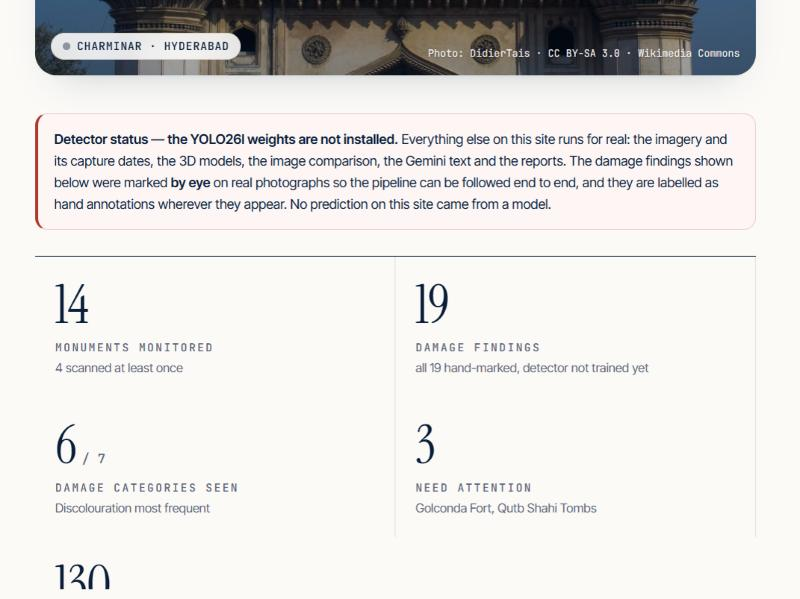
\includegraphics[width=\textwidth]{fig_dashboard_ledger.jpg}
\caption{Dashboard header. The detector status notice is unconditional while weights are absent, and the ledger beneath it states that all nineteen findings are hand-marked. Every figure shown is computed from the database.}
\label{fig:dashledger}
\end{figure}

\begin{figure}[H]
\centering
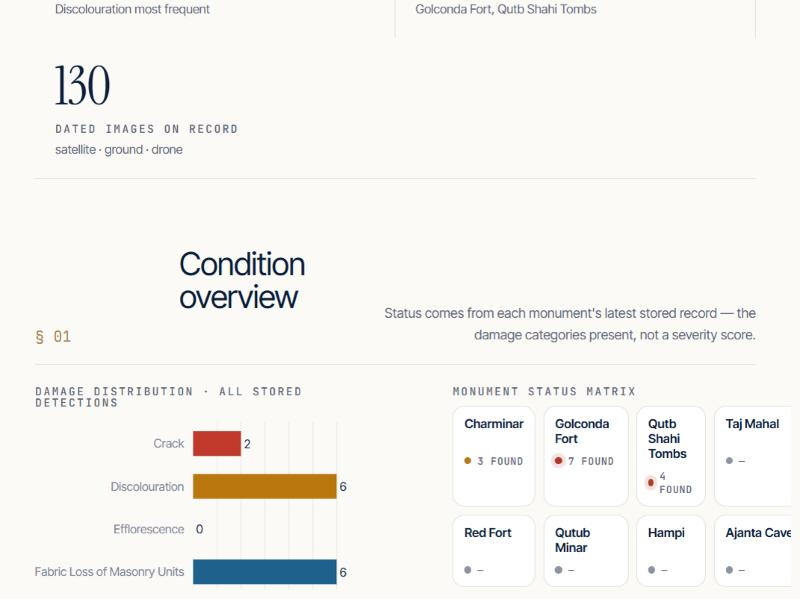
\includegraphics[width=\textwidth]{fig_dashboard_overview.jpg}
\caption{Condition overview. The distribution chart is annotated as hand-marked, and the status matrix derives each monument's state from the damage categories present rather than from detector confidence.}
\label{fig:dashoverview}
\end{figure}

\begin{figure}[H]
\centering
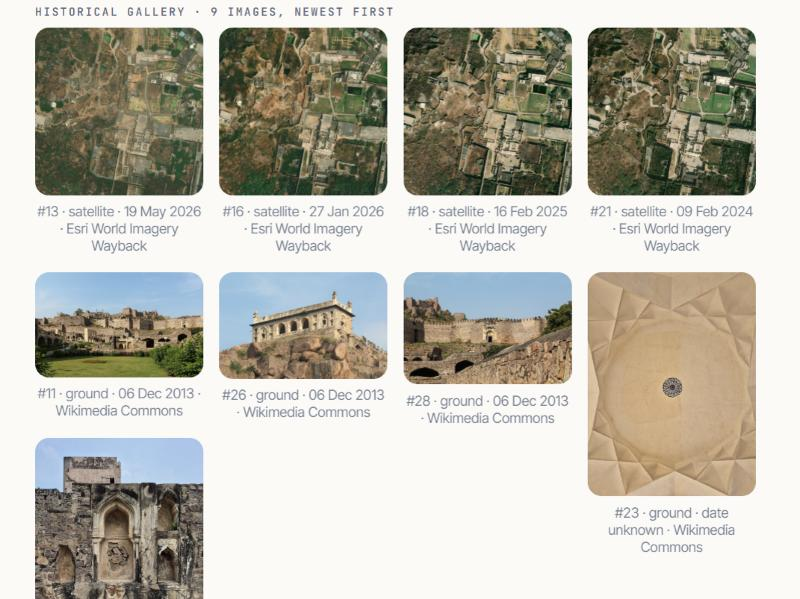
\includegraphics[width=\textwidth]{fig_imagery_gallery.jpg}
\caption{Section \S02 for Golconda Fort. Every thumbnail carries its kind, its capture date and its source; where a photographer did not state a date, the caption reads ``date unknown'' rather than substituting the upload date.}
\label{fig:imagerygallery}
\end{figure}

\begin{figure}[H]
\centering
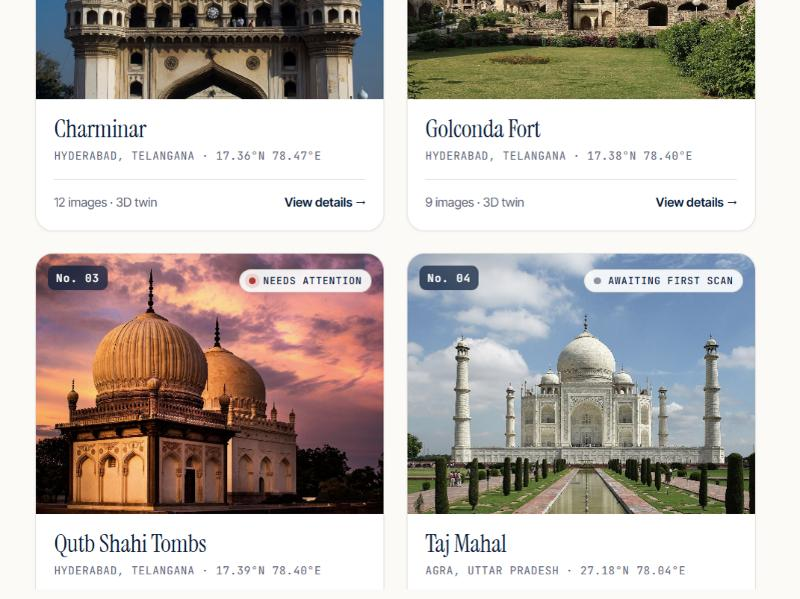
\includegraphics[width=\textwidth]{fig_monument_cards.jpg}
\caption{The monument index. Each card opens a dossier at its own URL, and carries the monument's location, its image count and whether a 3D twin is available.}
\label{fig:cards}
\end{figure}

\subsection{Software and Hardware}
Table~\ref{tab:stack} lists the implementation stack. Development was carried out on a Windows 11 machine without a CUDA GPU, which is why training was planned for a cloud notebook service. The deployed service runs on Google Cloud Run in the \texttt{asia-south1} region with 2 vCPU and 2\,GiB of memory, built from a container image defined in the repository.

\begin{table}[H]
\centering
\caption{Implementation stack}
\label{tab:stack}
\renewcommand{\arraystretch}{1.2}
{\footnotesize
\begin{tabular}{|l|l|}
\hline
\textbf{Concern} & \textbf{Technology} \\ \hline
Interface and routing & Streamlit, query-parameter routing, custom CSS theme \\ \hline
Detection & Ultralytics YOLO26l, PyTorch (CPU build) \\ \hline
3D visualisation & Three.js with GLTFLoader and OrbitControls \\ \hline
3D model generation & trimesh (parametric massing models) \\ \hline
Computer vision & OpenCV (ORB, RANSAC, CLAHE), NumPy \\ \hline
Storage & SQLAlchemy 2.0 over SQLite, PostgreSQL-compatible \\ \hline
Retrieval & LangChain, ChromaDB, sentence-transformers (all-MiniLM-L6-v2) \\ \hline
Language model & Google Gemini, with model fallback list \\ \hline
Reporting & ReportLab \\ \hline
Charts & Plotly (interface), Matplotlib (report figures) \\ \hline
Testing & pytest, twelve tests over a temporary database \\ \hline
Deployment & Docker image on Google Cloud Run, \texttt{asia-south1} \\ \hline
\end{tabular}}
\end{table}

\section{Performance Evaluation and Results}

\subsection{What Can and Cannot Be Evaluated at This Stage}
Honesty about results begins with saying which results exist. Because the detector is untrained, \textbf{no detection accuracy figures are reported in this document}. There is no mAP, no precision and no recall, because no model was run. Presenting numbers from a model trained on a different domain, or from the hand annotations, would be exactly the kind of claim this project was rebuilt to prevent.

What can be evaluated, and is reported below, is everything else: the coverage and dating of the image archive, the completeness of the 3D model set, the behaviour of the change-detection pipeline on real image pairs, the behaviour of the assistant, and the correctness of the software.

\subsection{Imagery Coverage}
The archive holds \textbf{130 images} across fourteen monuments, of which \textbf{119 carry a stated capture date}; the remaining eleven are ground photographs whose photographers did not state one, and are displayed as ``date unknown''. The split by source is 53 satellite scenes from Esri World Imagery Wayback and 77 ground photographs from Wikimedia Commons. Figure~\ref{fig:imagerybym} gives the per-monument breakdown.

Figure~\ref{fig:sattimeline} shows the satellite capture dates. The archive spans 2019 to 2026. Thirteen of the fourteen monuments hold four distinct capture dates each, which is enough to look at a trend rather than a single difference. Hampi holds only one, from March 2019: the Wayback releases covering that site repeat the same underlying pixels, and the acquisition routine stores a release only when its capture date differs from one already held, so no second observation exists to store. Hampi is therefore the one monument where change detection is currently impossible, and the interface shows this rather than padding the archive with duplicates. Ground sample distances reported by the metadata service range from 0.31 to 0.5\,m per pixel.

\begin{figure}[H]
\centering
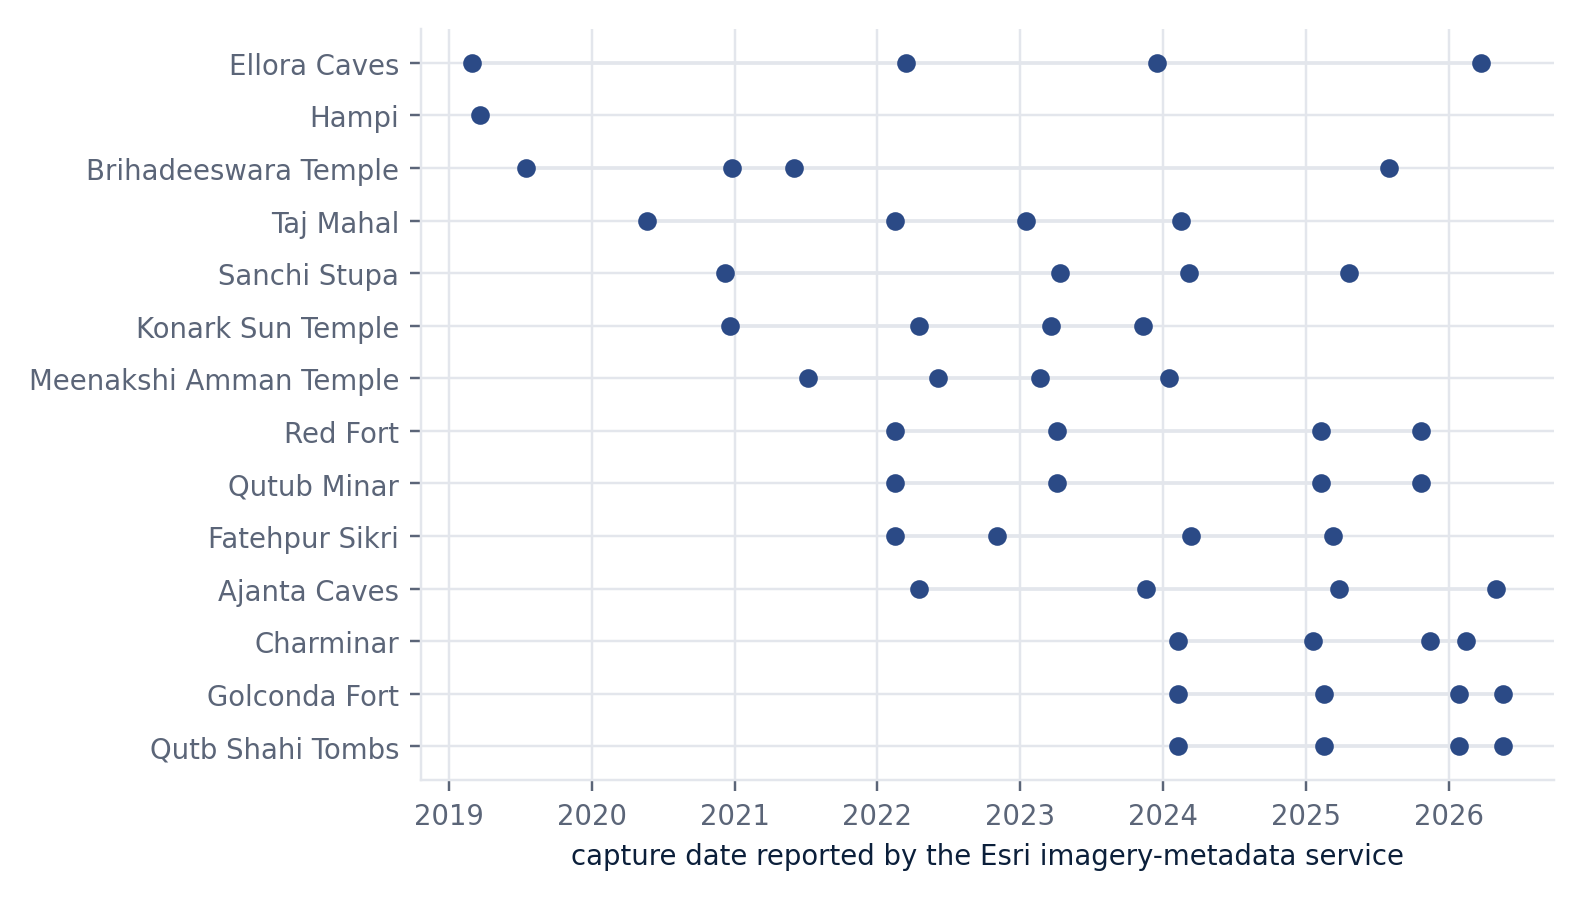
\includegraphics[width=\textwidth]{fig_satellite_timeline.png}
\caption{Satellite capture dates per monument, as reported by the Esri imagery-metadata service. Each point is a distinct capture date held in the archive; releases carrying identical pixels are not stored twice.}
\label{fig:sattimeline}
\end{figure}

\begin{figure}[H]
\centering
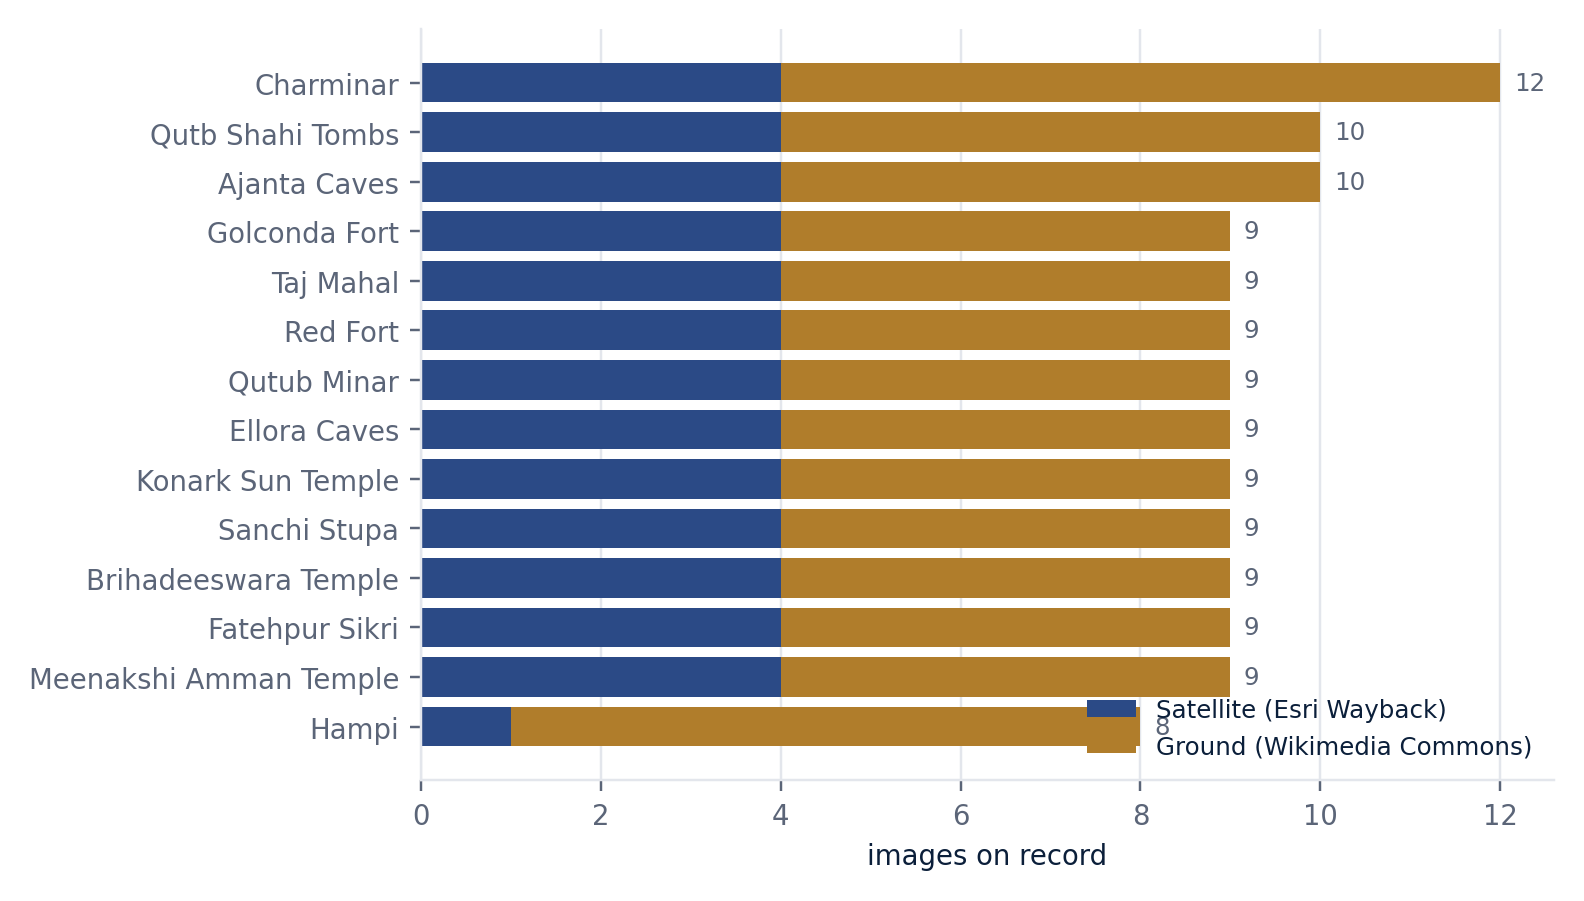
\includegraphics[width=\textwidth]{fig_imagery_by_monument.png}
\caption{Images on record per monument, split by source. Satellite scenes come from the Esri Wayback archive with true capture dates; ground photographs come from Wikimedia Commons with licence and attribution.}
\label{fig:imagerybym}
\end{figure}

The quantitative basis of the resolution argument is visible here. At $g = 0.31$\,m per pixel, a crack of width 2\,mm subtends $2 \times 10^{-3} / 0.31 \approx 0.0065$ of a pixel; a moss patch 5\,cm across subtends about 0.16 of a pixel. Neither is representable. This is why satellite imagery is routed to comparison and not to detection, and why the detection section displays a domain warning if a satellite image is selected.

\subsection{3D Model Coverage}
All fourteen monuments have a valid glTF model carrying embedded provenance, and this is enforced by an automated test that opens each file, parses its JSON chunk, checks that it contains mesh data and asserts that a provenance title is present. Three models are community reconstructions and eleven are parametric. Figures~\ref{fig:twincharminar} and \ref{fig:twin3d} show one of each, both with their provenance statements visible in the viewer.

\begin{figure}[H]
\centering
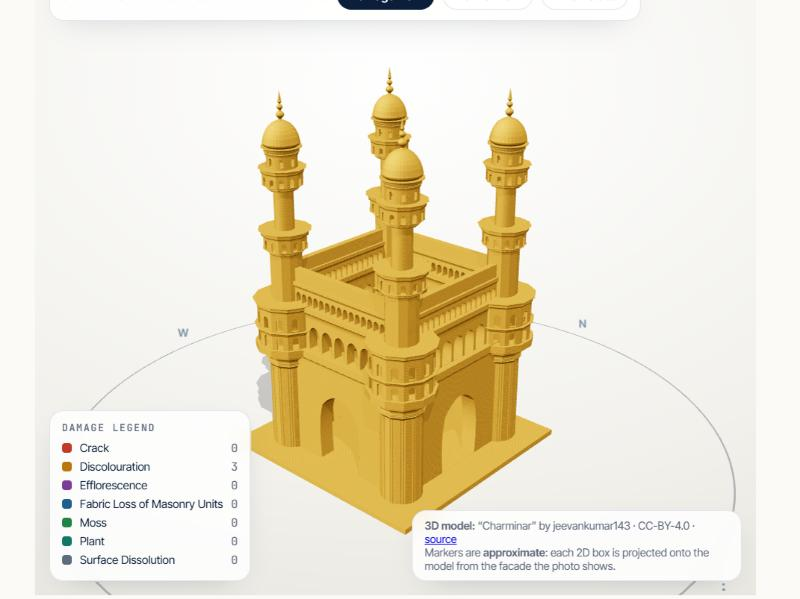
\includegraphics[width=0.84\textwidth]{fig_twin_charminar.jpg}
\caption{The Charminar twin: a freely licensed community reconstruction, with its author, licence and source link displayed in the viewer.}
\label{fig:twincharminar}
\end{figure}

\begin{figure}[H]
\centering
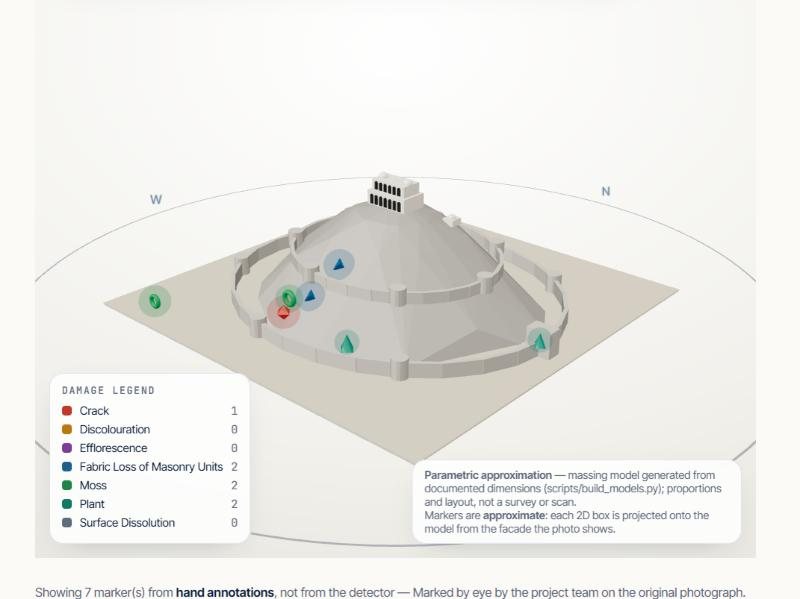
\includegraphics[width=0.84\textwidth]{fig_twin3d.jpg}
\caption{The Golconda Fort twin with seven findings projected onto it. The viewer states both that the model is a parametric approximation and that the marker positions are approximate.}
\label{fig:twin3d}
\end{figure}

\subsection{Change Detection}
The comparison pipeline was exercised on real image pairs from the archive and on controlled synthetic pairs in the test suite. On the synthetic pairs the behaviour is as specified: two identical scenes give $\bar{S} > 0.95$ with a changed fraction below 1\%, and a scene shifted by twelve pixels with an occluding block added is successfully registered and the block is recovered as a change region.

On real satellite pairs the pipeline exposes its own limits, which is the behaviour that was designed for. Figure~\ref{fig:comparison} shows a Golconda Fort pair captured years apart. Registration was \textbf{rejected}: only sixteen RANSAC inliers were found, below the threshold of thirty, because vegetation and seasonal colour change between the two dates destroy most ORB correspondences. The system therefore reports $\bar{S} = 0.201$ and a changed fraction of 58.9\% \textit{alongside an explicit statement that the images could not be aligned and the pixel differences are not meaningful}. A system that suppressed the failure would have reported a dramatic 58.9\% change at a monument where most of that figure is seasonal.

\begin{figure}[H]
\centering
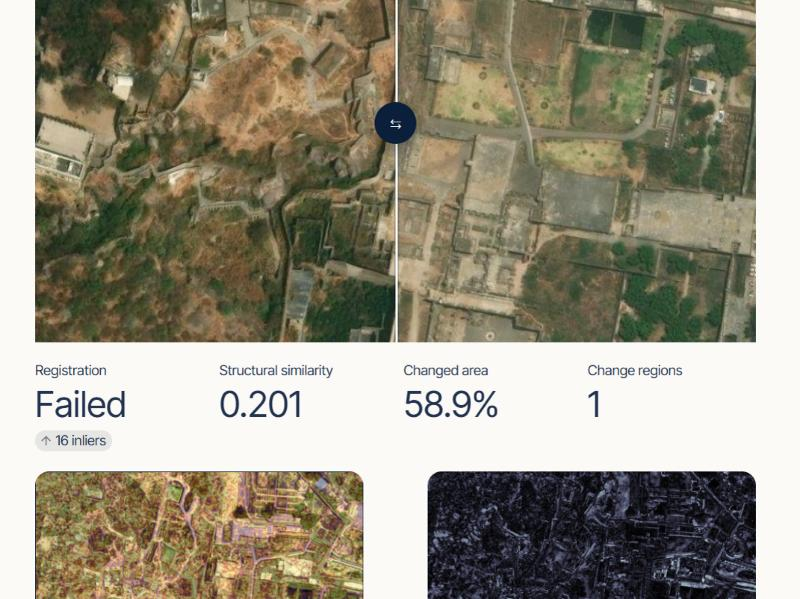
\includegraphics[width=\textwidth]{fig_comparison.jpg}
\caption{Multi-temporal comparison at Golconda Fort. The slider compares two dated satellite scenes; the metrics row reports that registration failed with sixteen inliers, so the similarity and change figures beside it are not to be read as deterioration.}
\label{fig:comparison}
\end{figure}

\subsection{Hand-Annotated Reference Set}
The nineteen hand annotations are distributed as shown in Figure~\ref{fig:damagedist}: six Discolouration, six Fabric Loss of Masonry Units, two Crack, two Moss, two Plant and one Surface Dissolution. Efflorescence has no example, because none was confidently identifiable in the available photographs --- recording nothing was preferred to recording a guess.

\begin{figure}[H]
\centering
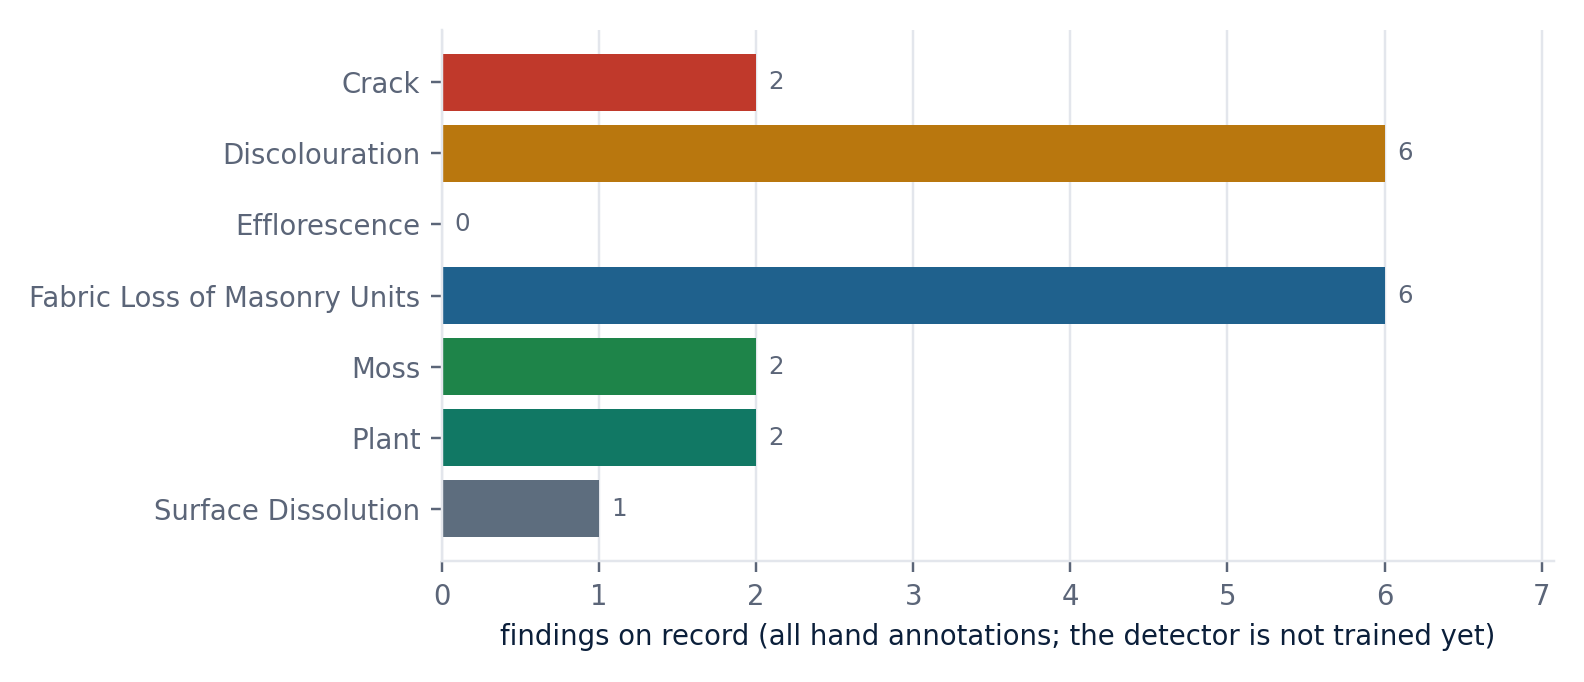
\includegraphics[width=\textwidth]{fig_damage_distribution.png}
\caption{Findings per damage category. All nineteen are hand annotations; the detector has not been trained. Efflorescence has no example because none was confidently identifiable in the available photographs.}
\label{fig:damagedist}
\end{figure}

\begin{figure}[H]
\centering
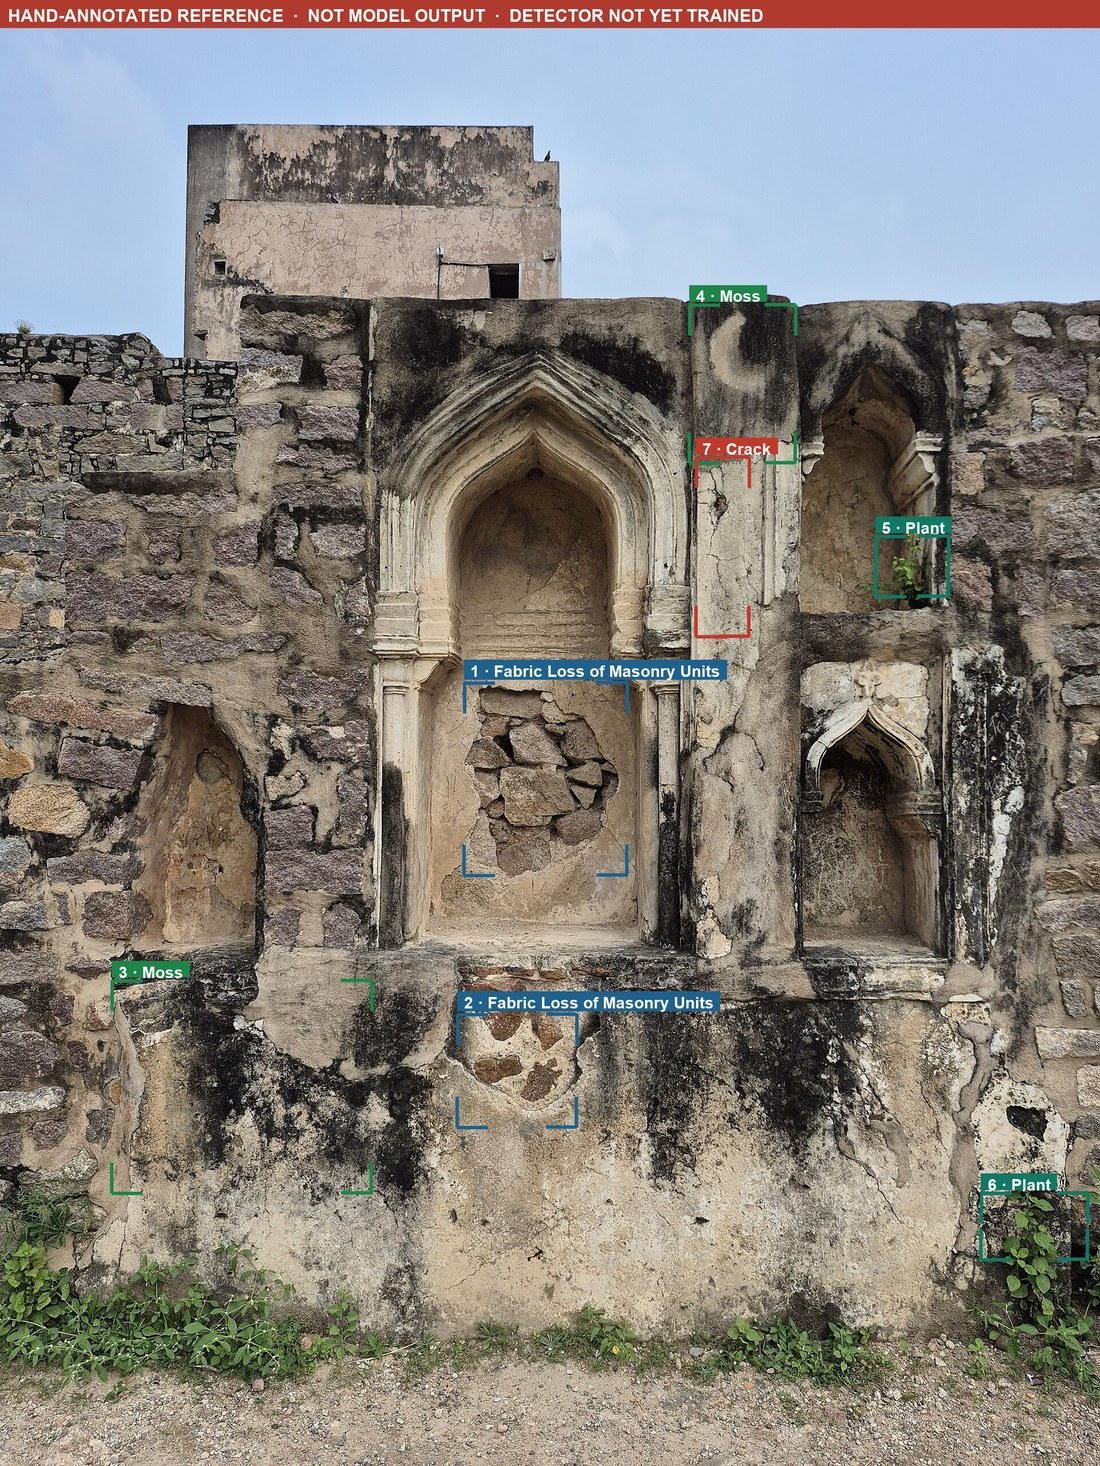
\includegraphics[width=0.74\textwidth]{fig_annotation_golconda.jpg}
\caption{Hand-annotated reference photograph of a ruined curtain wall at Golconda Fort: plaster and facing lost from the central niche exposing the rubble core, a second loss patch below the sill, biological growth on the damp lower wall, seedlings rooted in a niche and at the wall base, and a vertical fissure beside the niche arch. The banner is burnt into the stored image.}
\label{fig:annotgolconda}
\end{figure}

\begin{figure}[H]
\centering
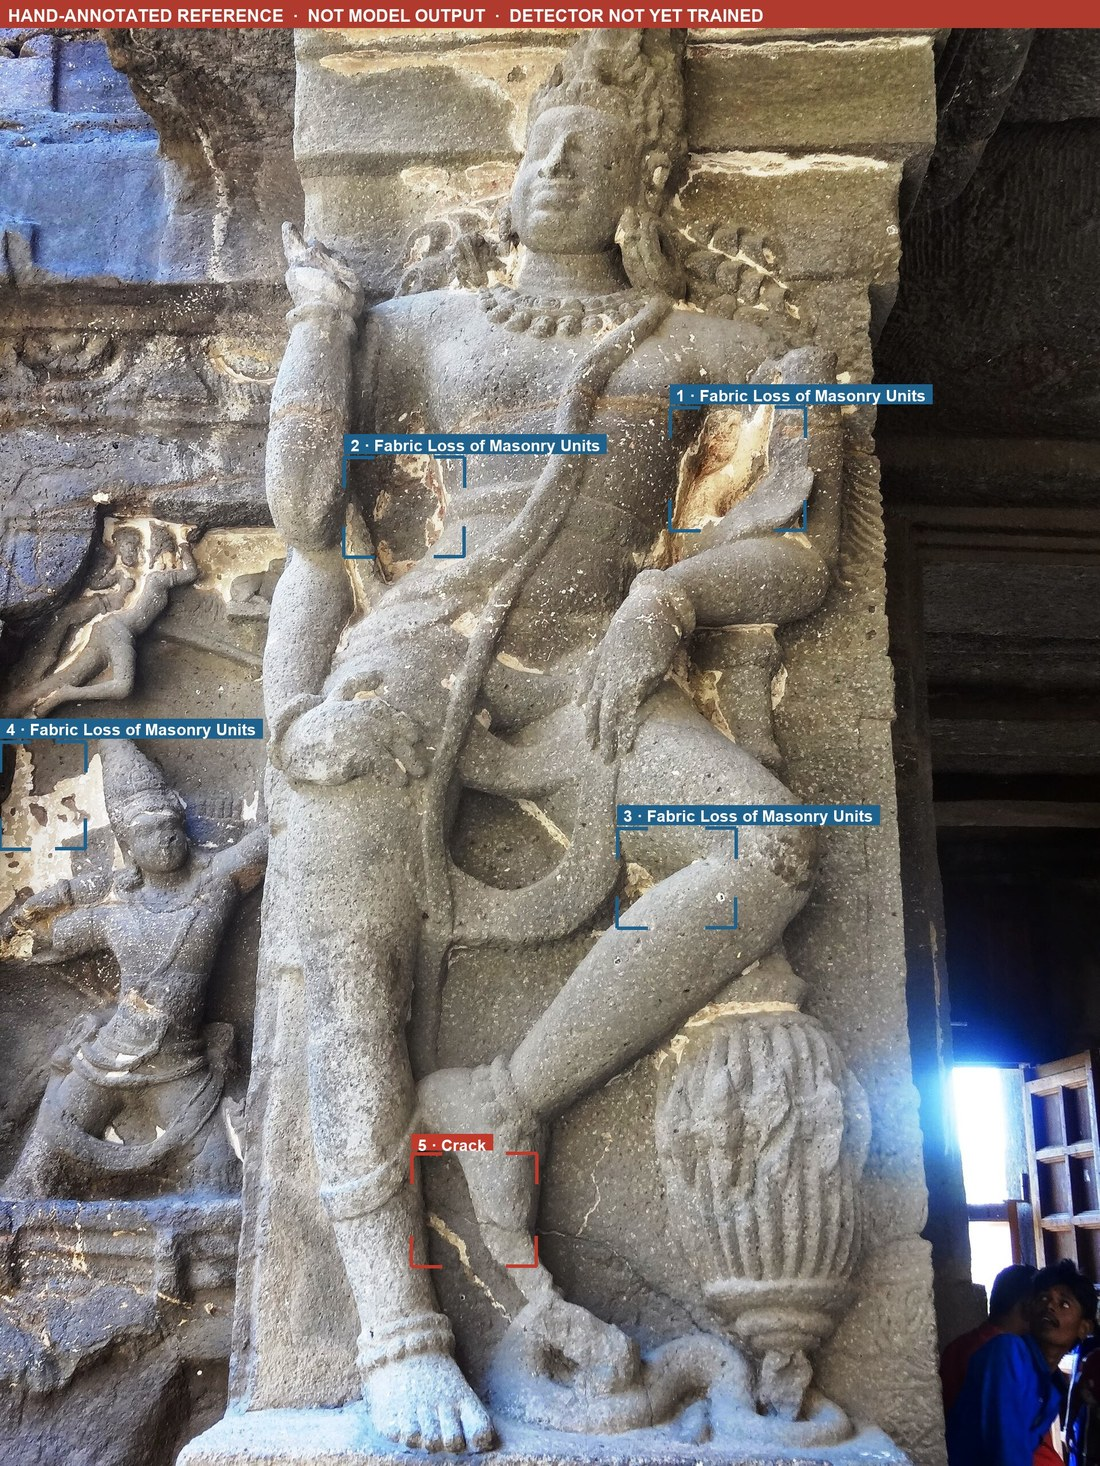
\includegraphics[width=0.74\textwidth]{fig_annotation_ellora.jpg}
\caption{A second hand-annotated photograph, inside a rock-cut cave at Ellora: four areas of stone loss on the relief and a diagonal fissure through the lower panel. The basalt substrate here is entirely different from the plastered rubble at Golconda, which is one reason a detector trained on concrete infrastructure cannot be assumed to transfer.}
\label{fig:annotellora}
\end{figure}

\begin{figure}[H]
\centering
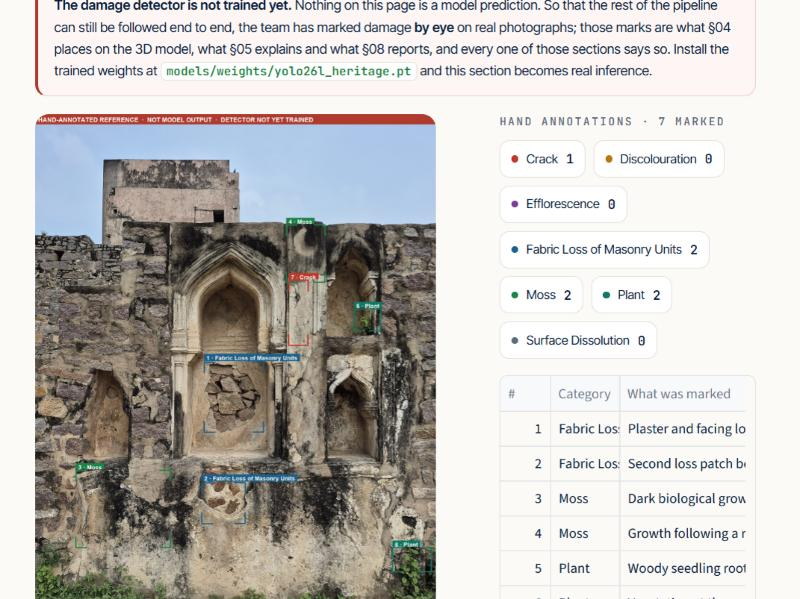
\includegraphics[width=\textwidth]{fig_detection_section.jpg}
\caption{Section \S03 while the detector is untrained. The notice, the burnt-in banner, the absence of any confidence column and the ``what was marked'' column together make the evidential status of the findings unambiguous.}
\label{fig:detection}
\end{figure}

\subsection{Explanation and Assistant Behaviour}
Both language-model surfaces were exercised without an API key configured, which is the harder case because it tests the fallback path. The explanation layer produced reference text for every category present and labelled it \textbf{general reference $\cdot$ Gemini unavailable}, with the card header reading ``hand annotation(s)'' rather than ``detection(s)'' and no confidence percentage, as shown in Figure~\ref{fig:explanations}.

\begin{figure}[H]
\centering
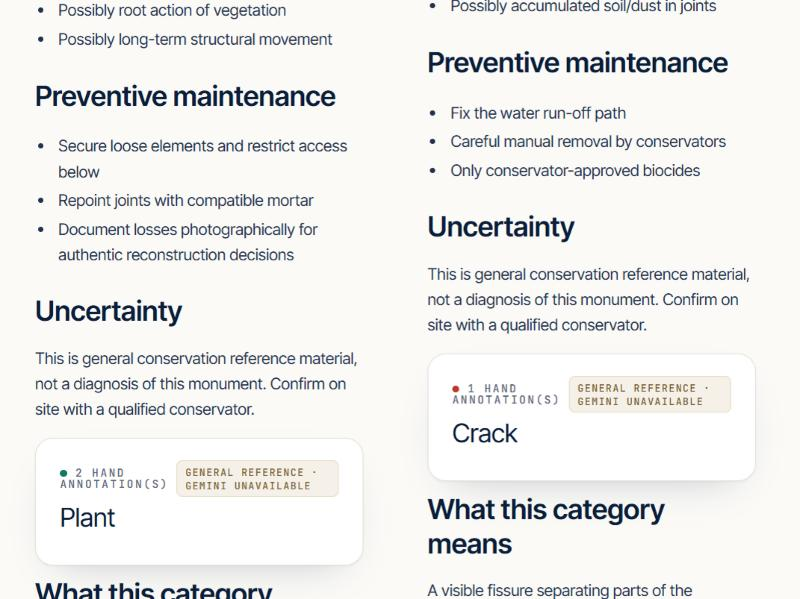
\includegraphics[width=\textwidth]{fig_explanations.jpg}
\caption{Section \S05. Each card names the number of hand annotations behind it and is tagged either as an AI-generated hypothesis or, as here, as general conservation reference because no API key is configured.}
\label{fig:explanations}
\end{figure}

The assistant was queried on the deployed service with ``What damage has been recorded here and what should be done about it?''. It returned the live monitoring context --- nine images on record, four satellite and five ground, the latest record, its producing method, and the categories marked --- labelled \textbf{retrieval only} with its retrieved sources named, and stated plainly that a Gemini key is not configured. Figure~\ref{fig:chatbot} shows the exchange. This is the intended degradation: the factual content is correct and sourced, and the absence of the generative layer is announced rather than hidden.

\begin{figure}[H]
\centering
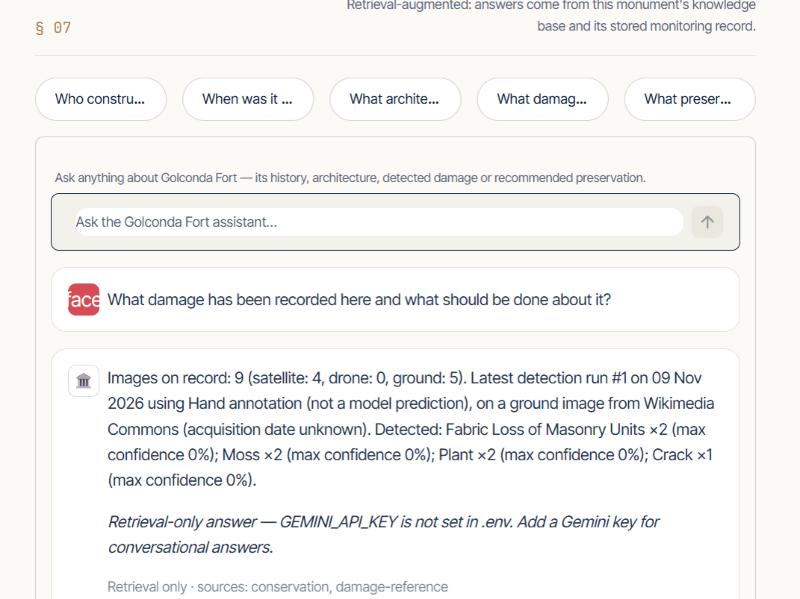
\includegraphics[width=\textwidth]{fig_chatbot.jpg}
\caption{Section \S07 on the deployed service. The answer is assembled from the monument's knowledge base and its live monitoring record; with no API key present the system returns retrieval only and says so.}
\label{fig:chatbot}
\end{figure}

\subsection{Software Quality and Audit Closure}
The test suite contains twelve tests, all passing, covering the registry, label normalisation including the numeric-class regression, the missing-weights error path, database statistics, the comparison pipeline on identical and shifted images, the explanation fallback, the validity and provenance of all fourteen 3D models, the well-formedness of the hand annotations, and the invariant that real inference never writes the demonstration flag.

Of the twenty-two defects recorded in the audit of the previous implementation, Table~\ref{tab:audit} lists the most consequential and their resolution. One requires action outside the code: the leaked Sentinel Hub client credentials were published in a public repository and must be revoked at the provider, since removing them from the source history does not invalidate them.

\begin{table}[H]
\centering
\caption{Principal audit findings and their resolution}
\label{tab:audit}
\renewcommand{\arraystretch}{1.2}
{\footnotesize
\begin{tabular}{|p{0.44\linewidth}|p{0.48\linewidth}|}
\hline
\textbf{Defect found in the previous implementation} & \textbf{Resolution} \\ \hline
Real API credentials committed to a public repository & Credentials removed; configuration read from an ignored environment file; \textbf{the leaked keys must still be revoked at the provider} \\ \hline
Report claimed YOLO26l; code loaded two different and absent weight files & One configurable weights path; class names read from the model and normalised \\ \hline
Three mutually inconsistent monument lists across modules & A single registry file of exactly fourteen monuments \\ \hline
Damage detector run on 10\,m-per-pixel satellite tiles & Detection restricted to close-range imagery; satellite routed to change detection; domain warning in the interface \\ \hline
Severity derived from detector confidence & Status derived from which categories were found; confidence shown only as confidence \\ \hline
3D markers placed on the model roof and presented as precise & Facade projection with ray casting, labelled approximate everywhere \\ \hline
Charminar model referenced at a non-existent path; Fatehpur Sikri model was a room photosphere & Correct static paths; all fourteen models present and provenance-tagged \\ \hline
``Fresh imagery'' control that returned an identical undated mosaic & Esri Wayback releases with true capture dates from the metadata service \\ \hline
Crash on import when the API key was absent & Graceful degradation with a labelled fallback on every AI surface \\ \hline
Retrieval for one monument only, with no access to monitoring data & One collection per monument plus live monitoring context in every answer \\ \hline
\end{tabular}}
\end{table}

\subsection{Discussion and Limitations}
The results support the system-level claims of the project: a monitoring record can be kept with real dates and sources at useful temporal density from free data; a lightweight per-monument twin is sufficient to place findings for review; and a pipeline can be built in which every output declares its own evidential status, including when a component is missing.

The limitations are stated plainly. \textbf{The detector does not exist yet}, so the central claim of automated damage detection is unproven in this report; what is delivered is the pipeline it will occupy, the training scripts and the integration test for the day it arrives. \textbf{The planned training substrate is out of domain}: CiF is concrete and steel infrastructure, and its authors report that specialised supervised models reach only about 25\% mAP even in domain \cite{farronato2026cif}, so expectations should be set accordingly. \textbf{Two categories have no training data at all}. \textbf{The hand annotations are a demonstration input, not a validation set}: nineteen boxes marked by the project team on four photographs are too few, and not independently verified, to measure anything. \textbf{3D placement is an assumption, not a measurement}, valid only for frontal, monument-filling photographs. \textbf{Change detection on multi-year satellite pairs frequently fails to register}, as Figure~\ref{fig:comparison} shows, so the current practical value of that section is in reporting the failure correctly rather than in quantifying change. Finally, \textbf{ground truth for deterioration is entirely absent}: nothing in this system has been checked against a conservator's field survey, which is the only evidence that would establish whether its findings are real.

% =====================================================================
\chapter{CONCLUSION}

This project set out to build a monitoring platform for Indian heritage monuments that a conservation officer could actually rely on --- one that keeps a dated record, localises damage on the building, and never claims more than its inputs support.

ChronicleHeritage keeps a permanent archive of 130 images across fourteen monuments, of which 119 carry a stated capture date. The 53 satellite scenes are drawn from the Esri World Imagery Wayback archive and each carries the true capture date of its pixels, obtained from Esri's imagery-metadata service rather than inferred from the download, giving a multi-temporal stack that runs from 2019 to 2026 at 0.31--0.5\,m per pixel. The 77 ground photographs carry their licence, photographer and stated date, and where a photographer did not state a date the system says so rather than substituting one. The damage vocabulary is derived from the ICOMOS-ISCS \textit{Illustrated Glossary on Stone Deterioration Patterns}, so that findings are recorded in terms a conservator already uses.

All fourteen monuments have a 3D twin, three of them freely licensed community reconstructions and eleven parametric massing models generated from documented dimensions by a reproducible script, each declaring its own provenance in the viewer. Damage findings are placed on the mesh by facade projection and ray casting and are labelled an approximate location wherever they appear, because a 2D box carries no depth. Multi-temporal comparison by ORB registration, RANSAC homography estimation and SSIM differencing supplies the site-level change view that satellite imagery can legitimately support, and reports its own failure --- as in the Golconda Fort pair, rejected at sixteen inliers --- rather than presenting unaligned pixel differences as deterioration.

The governing design decision of the rebuild was to make evidential status a property of the data rather than a convention of the interface. The previous implementation of this project ran a damage detector on ten-metre satellite pixels, derived severity from detector confidence, and placed every 3D marker on the roof of the model without qualification. Each of those is a claim the system could not support. In the rebuilt system every finding carries what produced it, every language-model output is labelled as hypothesis with its model named, every fallback announces itself, and an automated test asserts that real inference can never be marked as demonstration data.

That principle was tested by the project's own circumstances. The detector could not be trained: no openly licensed heritage dataset covering the seven categories was obtainable and the available free GPU services were down during the training window. Rather than display placeholder predictions, nineteen damage instances were marked by hand on four real photographs and are declared as hand annotations in the interface, the twin, the language-model prompt, the report, the dashboard and the stored image itself. The complete pipeline can therefore be demonstrated end to end without a single fabricated prediction, and those nineteen marks become the detector's first qualitative check on the day it is trained.

What this project delivers, then, is a working heritage monitoring platform with one component still to arrive, and a clear account of which of its outputs are measurements, which are estimates, which are retrieved facts and which are generated hypotheses. For a system intended to inform decisions about irreplaceable buildings, that distinction is not a caveat on the result; it is the result.

% =====================================================================
\chapter{FUTURE SCOPE}

\begin{enumerate}
    \item \textbf{Train and evaluate the detector.} Complete the fine-tuning run on the \textit{Cracks in the Foundation} dataset, report per-class mAP on a held-out split, and then run the trained model on the four hand-annotated photographs and compare its boxes against the human marks. Given the 25\% mAP that CiF's own authors report for specialised supervised models \cite{farronato2026cif}, the honest outcome to prepare for is a detector that is useful as a screening aid rather than a diagnostic instrument.
    \item \textbf{Build heritage-domain training data.} CiF is concrete and steel. The Darbhanga Fort brick masonry dataset \cite{darbhanga2025dataset} shows that a per-site heritage dataset is feasible to build. Collecting and labelling a few thousand images at the Hyderabad monuments, in the ICOMOS-ISCS vocabulary already used here, would close the domain gap and supply the two categories --- Plant and Surface Dissolution --- for which no open data currently exists.
    \item \textbf{Replace the 3D assumption with a measurement.} Register photographs to the models with Structure-from-Motion camera poses \cite{schoenberger2016sfm}; the calibration file is already structured to accept them. This would turn the approximate marker into a located one, and would allow the same physical defect to be tracked across photographs taken from different viewpoints.
    \item \textbf{Photogrammetric twins.} Replace the parametric massing models with photogrammetric reconstructions where field photography is possible, starting with a pilot at the Charminar, so that the twin carries real surface geometry rather than documented proportions.
    \item \textbf{Robust multi-temporal registration.} The current ORB and RANSAC pipeline fails on satellite pairs years apart because vegetation and season destroy correspondences. Mutual-information or learned registration, seasonal masking, and restricting comparison to the built footprint would make the change figures usable rather than merely honest.
    \item \textbf{Quantified progression.} Once registration is reliable and the detector exists, the same finding can be tracked across dates to give what conservation actually needs: not ``a crack is present'' but ``this crack has widened over eighteen months''.
    \item \textbf{Validation against field survey.} Arrange a joint inspection with a conservator at one monument and compare the system's findings against a professional condition survey. No claim about detection quality on real heritage fabric can be made until this is done.
    \item \textbf{Operational deployment.} Add scheduled re-acquisition so that each new Wayback release is checked automatically, role-based review in which an officer accepts or rejects each finding, and export in a format the Archaeological Survey of India's own record-keeping can accept.
\end{enumerate}

% Appendix and Code Attachments
\fontsize{10pt}{10pt}\selectfont

\begin{appendices}
\chapter{CODE ATTACHMENTS}

The complete source code, tests, audit and setup instructions are in the project repository. Five representative excerpts are reproduced below.

\section{Single-Point Class Normalisation}
From \texttt{core/damage\_reference.py}. This is the only place in the system that decides what a detector's label means. It accepts a class name, a spelling variant or a bare numeric index, and never raises on an unknown label.

\begin{lstlisting}[language=Python]
_CANON = {_norm(c): c for c in settings.DAMAGE_CLASSES}
_CANON.update({"discoloration": "Discolouration", "fabricloss": "Fabric Loss of Masonry Units",
               "fabriclossofmasonryunit": "Fabric Loss of Masonry Units", "masonryloss": "Fabric Loss of Masonry Units",
               "plants": "Plant", "vegetation": "Plant", "cracks": "Crack", "crak": "Crack",
               "salt": "Efflorescence", "efflorescense": "Efflorescence", "algae": "Moss",
               "surfacedissolution": "Surface Dissolution", "dissolution": "Surface Dissolution"})


def is_positional(label) -> bool:
    """True when `label` is a bare class id ("6", 6) rather than a class name."""
    return isinstance(label, (int, float)) or (isinstance(label, str) and label.strip().lstrip("-").isdigit())


def canonical(label) -> str:
    if is_positional(label):
        i = int(float(label))
        if 0 <= i < len(settings.DAMAGE_CLASSES):
            return settings.DAMAGE_CLASSES[i]
        return str(label)
    return _CANON.get(_norm(str(label)), str(label))


def color(label) -> str:
    """Never raises: an unknown label gets the neutral ink colour."""
    return DAMAGE.get(canonical(label), {}).get("color", "#0B1F3A")
\end{lstlisting}

\section{Real Satellite Capture Dates}
From \texttt{core/acquisition.py}. The Wayback archive gives dated releases; this function asks Esri's imagery-metadata service for the date the pixels over the monument were actually captured, which is what the record stores.

\begin{lstlisting}[language=Python]
def wayback_releases() -> list[dict]:
    cfg = S.get(settings.WAYBACK_CONFIG_URL, timeout=30).json()
    rel = []
    for k, v in cfg.items():
        m = re.search(r"(\d{4}-\d{2}-\d{2})", v["itemTitle"])
        if m:
            rel.append({"id": int(k), "date": datetime.strptime(m[1], "%Y-%m-%d"),
                        "tile": v["itemURL"], "meta": v.get("metadataLayerUrl", "")})
    return sorted(rel, key=lambda r: r["date"])


def _capture_meta(meta_url: str, lat: float, lon: float) -> dict | None:
    """Ask Esri's metadata service for the capture date of the pixels at (lat, lon)."""
    if not meta_url:
        return None
    for layer in range(0, 8):  # finest resolution layer first
        try:
            r = S.get(f"{meta_url}/{layer}/query", params={
                "geometry": f"{lon},{lat}", "geometryType": "esriGeometryPoint", "inSR": 4326,
                "spatialRel": "esriSpatialRelIntersects",
                "outFields": "SRC_DATE,SRC_RES,NICE_DESC,NICE_NAME",
                "returnGeometry": "false", "f": "json"}, timeout=20)
            feats = r.json().get("features") or []
        except Exception:
            continue
        if feats:
            a = feats[0]["attributes"]
            d = str(a.get("SRC_DATE") or "")
            date = datetime.strptime(d, "%Y%m%d") if re.fullmatch(r"\d{8}", d) else None
            return {"date": date, "res": a.get("SRC_RES"),
                    "provider": a.get("NICE_DESC") or "", "product": a.get("NICE_NAME") or ""}
    return None
\end{lstlisting}

\section{Registration That Reports Its Own Failure}
From \texttt{core/compare.py}. The homography is rejected unless it has enough inliers and a non-degenerate linear part; the caller then tells the user that pixel differences are not meaningful.

\begin{lstlisting}[language=Python]
def register(before, after):
    orb = cv2.ORB_create(5000)
    g1, g2 = cv2.cvtColor(before, cv2.COLOR_BGR2GRAY), cv2.cvtColor(after, cv2.COLOR_BGR2GRAY)
    k1, d1 = orb.detectAndCompute(g1, None)
    k2, d2 = orb.detectAndCompute(g2, None)
    if d1 is None or d2 is None or len(k1) < 20 or len(k2) < 20:
        return None, 0
    matches = cv2.BFMatcher(cv2.NORM_HAMMING).knnMatch(d2, d1, k=2)
    good = [m for m, n in (p for p in matches if len(p) == 2) if m.distance < 0.75 * n.distance]
    if len(good) < 25:
        return None, len(good)
    src = np.float32([k2[m.queryIdx].pt for m in good]).reshape(-1, 1, 2)
    dst = np.float32([k1[m.trainIdx].pt for m in good]).reshape(-1, 1, 2)
    H, mask = cv2.findHomography(src, dst, cv2.RANSAC, 4.0)
    inliers = int(mask.sum()) if mask is not None else 0
    det = abs(np.linalg.det(H[:2, :2])) if H is not None else 0
    if H is None or inliers < 30 or det < 0.2 or det > 5:
        return None, inliers          # caller reports: not aligned, differences not meaningful
    return H, inliers
\end{lstlisting}

\section{Hand Annotations Declared as Such}
From \texttt{core/annotation.py}. Corner brackets instead of solid boxes, no confidence percentage, and a banner burnt into the stored image so a screenshot cannot be mistaken for model output.

\begin{lstlisting}[language=Python]
REFERENCE_MODEL = "Hand annotation (not a model prediction)"
BANNER = "HAND-ANNOTATED REFERENCE  .  NOT MODEL OUTPUT  .  DETECTOR NOT YET TRAINED"


def render(image, dets):
    out = image.convert("RGB").copy()
    dr = ImageDraw.Draw(out)
    W, H = out.size
    w, arm = max(3, W // 300), max(18, W // 36)
    font = _font(max(15, W // 68))
    for i, d in enumerate(dets, 1):
        c = color(d["label"])
        x1, y1, x2, y2 = d["box"]
        for cx, sx in ((x1, 1), (x2, -1)):            # corner brackets, not a solid box
            for cy, sy in ((y1, 1), (y2, -1)):
                dr.line([(cx, cy), (cx + sx * arm, cy)], fill=c, width=w)
                dr.line([(cx, cy), (cx, cy + sy * arm)], fill=c, width=w)
        tag = f" {i} . {d['label']} "                 # no confidence: a hand mark has none
        ...
    bf = _font(max(16, W // 62))
    bh = dr.textbbox((0, 0), BANNER, font=bf)[3] + 20
    dr.rectangle([0, 0, W, bh], fill=(176, 58, 46))
    dr.text((14, 10), BANNER, fill="white", font=bf)
    return out
\end{lstlisting}

\section{The Test That Enforces the Honesty Rule}
From \texttt{tests/test\_core.py}. Real inference must never be recorded as demonstration data, and the dashboard must never count hand annotations as model findings.

\begin{lstlisting}[language=Python]
def test_real_runs_are_never_flagged_as_reference():
    img = db.add_image(monument_slug="sanchi-stupa", kind="ground", source="test", path="x.jpg")
    rid = db.save_run(img.id, "sanchi-stupa", "YOLO26l", "abc", 0.25, "south", "",
                      [{"label": "Crack", "confidence": 0.9, "box": [0, 0, 5, 5], "u": .2, "v": .3}])
    run = next(r for r in db.runs_for("sanchi-stupa") if r["id"] == rid)
    from core import annotation
    assert run["is_demo"] is False and not annotation.is_reference(run)
    assert db.global_stats()["reference_detections"] == 0


def test_hand_annotations_are_valid_and_clearly_marked():
    from core import annotation
    specs = annotation.load_specs()
    assert specs, "data/annotations.json has no annotations"
    for spec in specs:
        assert by_slug(spec["monument"]), spec["monument"]
        assert (settings.ROOT / spec["image"]).exists(), spec["image"]
        for b in spec["boxes"]:
            assert b["label"] in settings.DAMAGE_CLASSES, b["label"]
            x1, y1, x2, y2 = b["box"]
            assert 0 <= x1 < x2 <= 1 and 0 <= y1 < y2 <= 1, b
            assert b.get("note"), "every hand annotation says what was marked"
    assert "NOT MODEL OUTPUT" in annotation.BANNER
\end{lstlisting}

\end{appendices}

\fontsize{12pt}{12pt}\selectfont

%Change Bibliography to References
\renewcommand\bibname{BIBILOGRAPHY}
\clearpage
\phantomsection
\addcontentsline{toc}{chapter}{BIBILOGRAPHY}
\begin{thebibliography}{99}
\bibitem{icomos2008glossary} ICOMOS International Scientific Committee for Stone (ISCS), \emph{Illustrated Glossary on Stone Deterioration Patterns}, V. Verg\`es-Belmin (ed.), Monuments and Sites XV, ICOMOS, Paris, 2008.
\bibitem{cha2017deep} Y.-J. Cha, W. Choi, and O. B\"uy\"uk\"ozt\"urk, ``Deep Learning-Based Crack Damage Detection Using Convolutional Neural Networks,'' \emph{Computer-Aided Civil and Infrastructure Engineering}, vol.~32, no.~5, pp.~361--378, 2017.
\bibitem{redmon2016yolo} J. Redmon, S. Divvala, R. Girshick, and A. Farhadi, ``You Only Look Once: Unified, Real-Time Object Detection,'' in \emph{Proceedings of the IEEE Conference on Computer Vision and Pattern Recognition (CVPR)}, pp.~779--788, 2016.
\bibitem{ultralytics2023yolo} G. Jocher, A. Chaurasia, and J. Qiu, ``Ultralytics YOLO,'' software, 2023. [Online]. Available: \url{https://github.com/ultralytics/ultralytics}
\bibitem{dorafshan2018sdnet} S. Dorafshan, R. J. Thomas, and M. Maguire, ``SDNET2018: An annotated image dataset for non-contact concrete crack detection using deep convolutional neural networks,'' \emph{Data in Brief}, vol.~21, pp.~1664--1668, 2018.
\bibitem{farronato2026cif} D. Farronato, M. Avogaro, \emph{et al.}, ``Cracks in the Foundation: A Civil Infrastructure Dataset to Challenge Vision Foundation Models,'' in \emph{Advances in Neural Information Processing Systems (NeurIPS), Datasets and Benchmarks Track}, 2026. arXiv:2605.18413. Dataset: \url{https://huggingface.co/datasets/ibm-research/cif-dataset}
\bibitem{darbhanga2025dataset} ``Brick Masonry Surface Damage Dataset Collected from Battledore of the Darbhanga Fort (A Cultural Heritage) for Automatic Damage Detection,'' Mendeley Data, V1, 2025. doi:\,10.17632/s6t5nn73bm.1
\bibitem{gil2024hbim} A. Gil, \emph{et al.}, ``Machine and Deep Learning Implementations for Heritage Building Information Modelling: A Critical Review of Theoretical and Applied Research,'' \emph{ACM Journal on Computing and Cultural Heritage}, 2024.
\bibitem{tootoonchi2026dt} A. Tootoonchi and M. Hess, ``Heritage Digital Twins: A Scoping Review of Peer-Reviewed Studies 2020--2025,'' \emph{ISPRS Annals of the Photogrammetry, Remote Sensing and Spatial Information Sciences}, vol.~XI-4, pp.~435--442, 2026.
\bibitem{banfi2026hbim} F. Banfi and Y. Liu, ``HBIM in Digital Heritage 2015--2025: Extended Reality, Artificial Intelligence, Semantic Segmentation and Digital Twins,'' \emph{Applied Sciences}, vol.~16, art.~906, 2026.
\bibitem{luo2019remote} L. Luo, X. Wang, H. Guo, R. Lasaponara, X. Zong, N. Masini, \emph{et al.}, ``Airborne and spaceborne remote sensing for archaeological and cultural heritage applications: A review of the century (1907--2017),'' \emph{Remote Sensing of Environment}, vol.~232, art.~111280, 2019.
\bibitem{tapete2017sar} D. Tapete and F. Cigna, ``Trends and perspectives of space-borne SAR remote sensing for archaeological landscape and cultural heritage applications,'' \emph{Journal of Archaeological Science: Reports}, vol.~14, pp.~716--726, 2017.
\bibitem{li2026review} Y. Li, F. Chiabrando, and G. Sammartano, ``Machine and Deep Learning for Cultural Heritage Conservation: A Bibliometric and Task-Oriented Review,'' \emph{Remote Sensing}, 2026.
\bibitem{rublee2011orb} E. Rublee, V. Rabaud, K. Konolige, and G. Bradski, ``ORB: An efficient alternative to SIFT or SURF,'' in \emph{Proceedings of the IEEE International Conference on Computer Vision (ICCV)}, pp.~2564--2571, 2011.
\bibitem{fischler1981ransac} M. A. Fischler and R. C. Bolles, ``Random Sample Consensus: A Paradigm for Model Fitting with Applications to Image Analysis and Automated Cartography,'' \emph{Communications of the ACM}, vol.~24, no.~6, pp.~381--395, 1981.
\bibitem{wang2004ssim} Z. Wang, A. C. Bovik, H. R. Sheikh, and E. P. Simoncelli, ``Image Quality Assessment: From Error Visibility to Structural Similarity,'' \emph{IEEE Transactions on Image Processing}, vol.~13, no.~4, pp.~600--612, 2004.
\bibitem{zuiderveld1994clahe} K. Zuiderveld, ``Contrast Limited Adaptive Histogram Equalization,'' in \emph{Graphics Gems IV}, Academic Press, pp.~474--485, 1994.
\bibitem{bradski2000opencv} G. Bradski, ``The OpenCV Library,'' \emph{Dr. Dobb's Journal of Software Tools}, 2000.
\bibitem{schoenberger2016sfm} J. L. Sch\"onberger and J.-M. Frahm, ``Structure-from-Motion Revisited,'' in \emph{Proceedings of the IEEE Conference on Computer Vision and Pattern Recognition (CVPR)}, pp.~4104--4113, 2016.
\bibitem{lewis2020rag} P. Lewis, E. Perez, A. Piktus, F. Petroni, V. Karpukhin, N. Goyal, \emph{et al.}, ``Retrieval-Augmented Generation for Knowledge-Intensive NLP Tasks,'' in \emph{Advances in Neural Information Processing Systems (NeurIPS)}, 2020.
\bibitem{reimers2019sbert} N. Reimers and I. Gurevych, ``Sentence-BERT: Sentence Embeddings using Siamese BERT-Networks,'' in \emph{Proceedings of EMNLP-IJCNLP}, pp.~3982--3992, 2019.
\bibitem{esriwayback} Esri, ``World Imagery Wayback,'' online archive of historical World Imagery releases. [Online]. Available: \url{https://livingatlas.arcgis.com/wayback/}
\bibitem{wikicommons} Wikimedia Foundation, ``Wikimedia Commons,'' freely licensed media repository. [Online]. Available: \url{https://commons.wikimedia.org/}
\bibitem{asi} Archaeological Survey of India, Ministry of Culture, Government of India. [Online]. Available: \url{https://asi.nic.in/}
\bibitem{gemini2024} Google DeepMind, ``Gemini,'' large language model family. [Online]. Available: \url{https://deepmind.google/technologies/gemini/}
\end{thebibliography}


\end{document}
